\documentclass{article} % A4 paper and 11pt font size
\setcounter{secnumdepth}{0}

\usepackage{amssymb, amsmath, amsfonts}
\usepackage{moreverb}
\usepackage{multicol}
\usepackage{graphicx}
\usepackage{enumerate}
\usepackage{caption}
\usepackage{nicefrac}
\usepackage{graphics}
\usepackage[margin=1in]{geometry}
\usepackage{tocloft}
\renewcommand{\cftsecleader}{\cftdotfill{\cftdotsep}}
\usepackage{array}
\usepackage{arydshln}
\usepackage{float}
\usepackage{subcaption}
\usepackage{csquotes}
\usepackage{placeins}
\usepackage{verbatim}
\usepackage{hyperref}
\usepackage{textcomp}
\usepackage[makeroom]{cancel}
\usepackage{bbold}
\usepackage{scrextend}
\usepackage{alltt}
\usepackage[utf8]{inputenc}
\usepackage{listings}
\usepackage{color}
\usepackage{physics}
\usepackage{mathtools}
\usepackage[normalem]{ulem}
\usepackage{amsthm}
\usepackage{tikz}
\usetikzlibrary{positioning}
\usetikzlibrary{arrows}
\usepackage{pgfplots}
\usepackage{bigints}
\allowdisplaybreaks
\pgfplotsset{compat=1.12}

\theoremstyle{plain}
\newtheorem*{theorem*}{Theorem}
\newtheorem{theorem}{Theorem}
\newtheorem*{lemma*}{Lemma}
\newtheorem{lemma}{Lemma}

\definecolor{verbgray}{gray}{0.9}
% \definecolor{dkgreen}{green}{0.9}

\lstdefinestyle{PythonCode}{%
  language=Python,
  backgroundcolor=\color{verbgray},
  keywordstyle=\color{blue},      % keyword style
  keywordstyle=[2]\color{blue},   % keyword style
  commentstyle=\color{magenta},   % comment style
  stringstyle=\color{olive},      % string literal styleframe=single,
  numberstyle=\color{black},      % string literal styleframe=single,
  framerule=0pt,
  numbers=left,
  stepnumber=1,
  firstnumber=1,
  showspaces=false,
  basicstyle=\ttfamily}

\lstset{style=PythonCode}

\makeatletter
\newcommand{\BIGG}{\bBigg@{3}}
\newcommand{\vast}{\bBigg@{4}}
\newcommand{\Vast}{\bBigg@{5}}
\makeatother

\newenvironment{definition}[1][Definition]{\begin{trivlist}
\item[\hskip \labelsep {\bfseries #1}]}{\end{trivlist}}

\newcommand{\dy}{\partial_y}
\newcommand{\dyy}{\partial_{yy}}
\newcommand{\dxx}{\partial_{xx}}
\newcommand{\dxy}{\partial_{xy}}
\newcommand{\dyyy}{\partial_{yyy}}
\newcommand{\dxxx}{\partial_{xxx}}
\newcommand{\dx}{\partial_x}
\newcommand{\E}{\varepsilon}
\def\Rl{\mathbb{R}}
\def\Cx{\mathbb{C}}

\newcommand{\Ei}{\text{Ei}}

\usepackage[T1]{fontenc} % Use 8-bit encoding that has 256 glyphs
\usepackage{fourier} % Use the Adobe Utopia font for the document - comment this line to return to the LaTeX default
\usepackage[english]{babel} % English language/hyphenation

\usepackage{sectsty} % Allows customizing section commands
\allsectionsfont{\centering \normalfont\scshape} % Make all sections centered, the default font and small caps

\usepackage{fancyhdr} % Custom headers and footers
\pagestyle{fancy} % Makes all pages in the document conform to the custom headers and footers
\fancyhead[L]{\bf Sam Fleischer}
\fancyhead[C]{\bf UC Davis \\ Numerical Solutions of Differential Equations (MAT228B)} % No page header - if you want one, create it in the same way as the footers below
\fancyhead[R]{\bf Winter 2017}

\fancyfoot[L]{\bf } % Empty left footer
\fancyfoot[C]{\bf \thepage} % Empty center footer
\fancyfoot[R]{\bf } % Page numbering for right footer
\renewcommand{\headrulewidth}{0pt} % Remove header underlines
\renewcommand{\footrulewidth}{0pt} % Remove footer underlines
\setlength{\headheight}{25pt} % Customize the height of the header

\newcommand{\VEC}[2]{\left\langle #1, #2 \right\rangle}
\newcommand{\ran}{\text{\rm ran }}
\newcommand{\Hilb}{\mathcal{H}}
\newcommand{\lap}{\Delta}

\newcommand{\Dx}{\Delta x}
\newcommand{\Dt}{\Delta t}

\newcommand{\littleo}[1]{\text{\scriptsize$\mathcal{O}$}\qty(#1)}

\DeclareMathOperator*{\esssup}{\text{ess~sup}}

\newcommand{\problem}[2]{
\vspace{.375cm}
\boxed{\begin{minipage}{\textwidth}
    \section{\bf #1}
    #2
\end{minipage}}
}

\numberwithin{equation}{section} % Number equations within sections (i.e. 1.1, 1.2, 2.1, 2.2 instead of 1, 2, 3, 4)
\numberwithin{figure}{section} % Number figures within sections (i.e. 1.1, 1.2, 2.1, 2.2 instead of 1, 2, 3, 4)
\numberwithin{table}{section} % Number tables within sections (i.e. 1.1, 1.2, 2.1, 2.2 instead of 1, 2, 3, 4)

\setlength\parindent{0pt} % Removes all indentation from paragraphs - comment this line for an assignment with lots of text

\newcommand{\horrule}[1]{\rule{\linewidth}{#1}} % Create horizontal rule command with 1 argument of height

\title{ 
\normalfont \normalsize 
\textsc{UC Davis, Numerical Solutions of Differential Equations (MAT 228B), Winter 2017} \\ [25pt] % Your university, school and/or department name(s)
\horrule{2pt} \\[01.4cm] % Thin top horizontal rule
\Huge Homework \#1 \\ % The assignment title
\horrule{2pt} \\[0.5cm] % Thick bottom horizontal rule
}

\author{\huge Sam Fleischer} % Your name

\date{December 9, 2016} % Today's date or a custom date

\begin{document}\thispagestyle{empty}

\maketitle % Print the title

\makeatletter
\@starttoc{toc}
\makeatother

\pagebreak

\problem{Problem 1}{Consider the advection equation $$u_t + au_x = 0$$ on the interval $[0,1)$ with periodic boundary conditions.  Space is discretized as $x_j = j\Delta x$ for $j = 0,\dots,N-1$ so that $\Delta x = \nicefrac{1}{N}$.  Discretize the spatial derivative with the second-order centered difference operator.
\begin{enumerate}[\ \ (a)]
    \item For simplicity, assume $N$ is odd.  The eigenvectors of the centered difference operator are $$v_j^k = \exp(2\pi ikx_j),$$ for $k = -\frac{N-1}{2},\dots,\frac{N-1}{2}$.  Compute the eigenvalues.
    \item Derivate a time step restriction on a method-of-lines approach which uses classical fourth-order Runge-Kutta for time stepping.
\end{enumerate}}

\begin{enumerate}[\ \ (a)]
    \item The eigenvalues $\lambda_k$ of the centered difference operator satisfy
    \begin{align*}
        \frac{v_{j+1}^k - v_{j-1}^k}{2\Delta x} &= \lambda v_j^k \\
        \frac{\exp[2\pi i k(x_j + \Delta x)] - \exp[2\pi i k(x_j - \Delta x)]}{2\Delta x} &= \lambda_k \exp[2\pi i k x_j] \\
        \cancelto{}{\exp[2\pi ikx_j]}\frac{\exp[2\pi i k \Delta x] - \exp[-2\pi i k \Delta x]}{2\Delta x} &= \lambda_k \cancelto{}{\exp[2\pi i k x_j]}
    \end{align*}
    Thus, $\boxed{\lambda_k = \dfrac{\sin(2\pi k \Delta x)}{\Delta x}i}$.  Note they are purely imaginary.
    \item The Classical RK4 algorithm is
    \begin{align*}
        y_1^* &= y^n \\
        y_2^* &= y^n + \frac{\Dt}{2}f\qty(y_1^*,t_n)\\
        y_3^* &= y^n + \frac{\Dt}{2}f\qty(y_2^*,t_n + \frac{\Dt}{2}) \\
        y_4^* &= y^n + \Dt f\qty(y_3^*,t_n + \frac{\Dt}{2}) \\
        y^{n+1} &= y^n + \frac{\Dt}{6}\qty(f\qty(y_1^*,t_n) + 2f\qty(y_2^*,t_n + \frac{\Dt}{2}) + 2f\qty(y_3^*,t_n + \frac{\Dt}{2}) + f\qty(y_4^*,t_n + \Dt))
    \end{align*}
    Next we set $f(y,t) = a\lambda y$ and get
    \begin{align*}
        y_2^* &= y^n + a\lambda\frac{\Dt}{2}y^n = y^n\qty(1 + a\lambda\frac{\Dt}{2})\\
        y_3^* &= y^n + a\lambda\frac{\Dt}{2}\qty(y^n + a\lambda\frac{\Dt}{2}y^n) = y^n\qty(1 + \qty(a\lambda\frac{\Dt}{2}) + \qty(a\lambda\frac{\Dt}{2})^2) \\
        y_4^* &= y^n + a\lambda\Dt y^n\qty(1 + \qty(a\lambda\frac{\Dt}{2}) + \qty(a\lambda\frac{\Dt}{2})^2) = y^n\qty(1 + a\lambda\Dt + \frac{(a\lambda\Dt)^2}{2} + \frac{(a\lambda\Dt)^3}{2^2}) \\
        y^{n+1} &= y^n + \frac{\Dt}{6}\qty(a\lambda y^n + 2a\lambda y^n\qty(1 + a\lambda\frac{\Dt}{2}) + 2a\lambda y^n\qty(1 + a\lambda\frac{\Dt}{2} + (a\lambda)^2\frac{\Dt^2}{2^2}) + a\lambda y^n\qty(1 + a\lambda\Dt + (a\lambda)^2\frac{\Dt^2}{2} + (a\lambda)^3\frac{\Dt^3}{2^2})) \\
        &= y^n\qty(1 + \frac{\Dt}{6}\qty(a\lambda + 2a\lambda + (a\lambda)^2\Dt + 2a\lambda + (a\lambda)^2\Dt + \frac{1}{2}(a\lambda)^3\Dt^2 + a\lambda + (a\lambda)^2\Dt + \frac{1}{2}(a\lambda)^3\Dt^2 + \frac{1}{4}(a\lambda)^4\Dt^3)) \\
        &= y^n\qty(1 + a\lambda\Dt + \frac{1}{2!}\qty(a\lambda\Dt)^2 + \frac{1}{3!}\qty(a\lambda\Dt)^3 + \frac{1}{4!}\qty(a\lambda\Dt)^4)
    \end{align*}
    Setting $z = a\lambda\Dt$, we get $y^{n+1} = R(z)y^n$ where $R(z) = 1 + z + \frac{z^2}{2!} + \frac{z^3}{3!} + \frac{z^4}{4!}$.  Since $\lambda$ are purely imaginary, set $z = \lambda a\Dt = im$ where $m\in\Rl$.  So,
    \begin{align*}
        \abs{1 + im - \frac{1}{2}m^2 - i\frac{1}{6}m^3 + \frac{1}{24}m^4}&< 1 \\
        \abs{\qty(1 - \frac{m^2}{2} + \frac{m^4}{24}) + \qty(m - \frac{m^3}{6})i} &< 1 \\
        \implies \qty(1 - \frac{m^2}{2} + \frac{m^4}{24})^2 + \qty(m - \frac{m^3}{6})^2 &< 1 \\
        \implies 1 + \frac{m^4}{4} + \frac{m^8}{576} - m^2 + \frac{m^4}{12} - \frac{m^6}{24} + m^2 + \frac{m^6}{36} - \frac{m^4}{3} &< 1 \\
        \frac{m^8}{576} - \frac{m^6}{72} &< 0 \\
        \frac{m^2}{8} - 1 &< 0 \\
        \implies \abs{m} &< 2\sqrt{2}
    \end{align*}
    This gives $\frac{\sin(2\pi k\Dx)}{\Dx}a\Dt \leq 2\sqrt{2}$, but $\sin(2\pi k\Dx) \leq 1$, so
    \begin{align*}
        \Dt \leq \frac{2\sqrt{2}\Dx}{a}
    \end{align*}
    is the stability condition.
\end{enumerate}









\pagebreak
\problem{Problem 2}{Consider the following PDE.
\begin{gather*}
    u_t = 0.01u_{xx} + 1 - \exp(-t),\qquad 0 < x < 1 \\
    u(0,t) = 0\qquad u(1,t) = 0\\
    u(x,0) = 0
\end{gather*}
Write a program to solve the problem using Crank-Nicolson up to time $t = 1$ and perform a refinement study that demonstrates that the method is second-order accurate in space and time.}

The following figures show the differential equation solved from $t=0$ to $t=1$ for $(\Dx,\Dt) = \qty(2^{-3},2^{-3}),\dots,\qty(2^{-10},2^{-10})$.

\begin{minipage}{0.5\textwidth}
    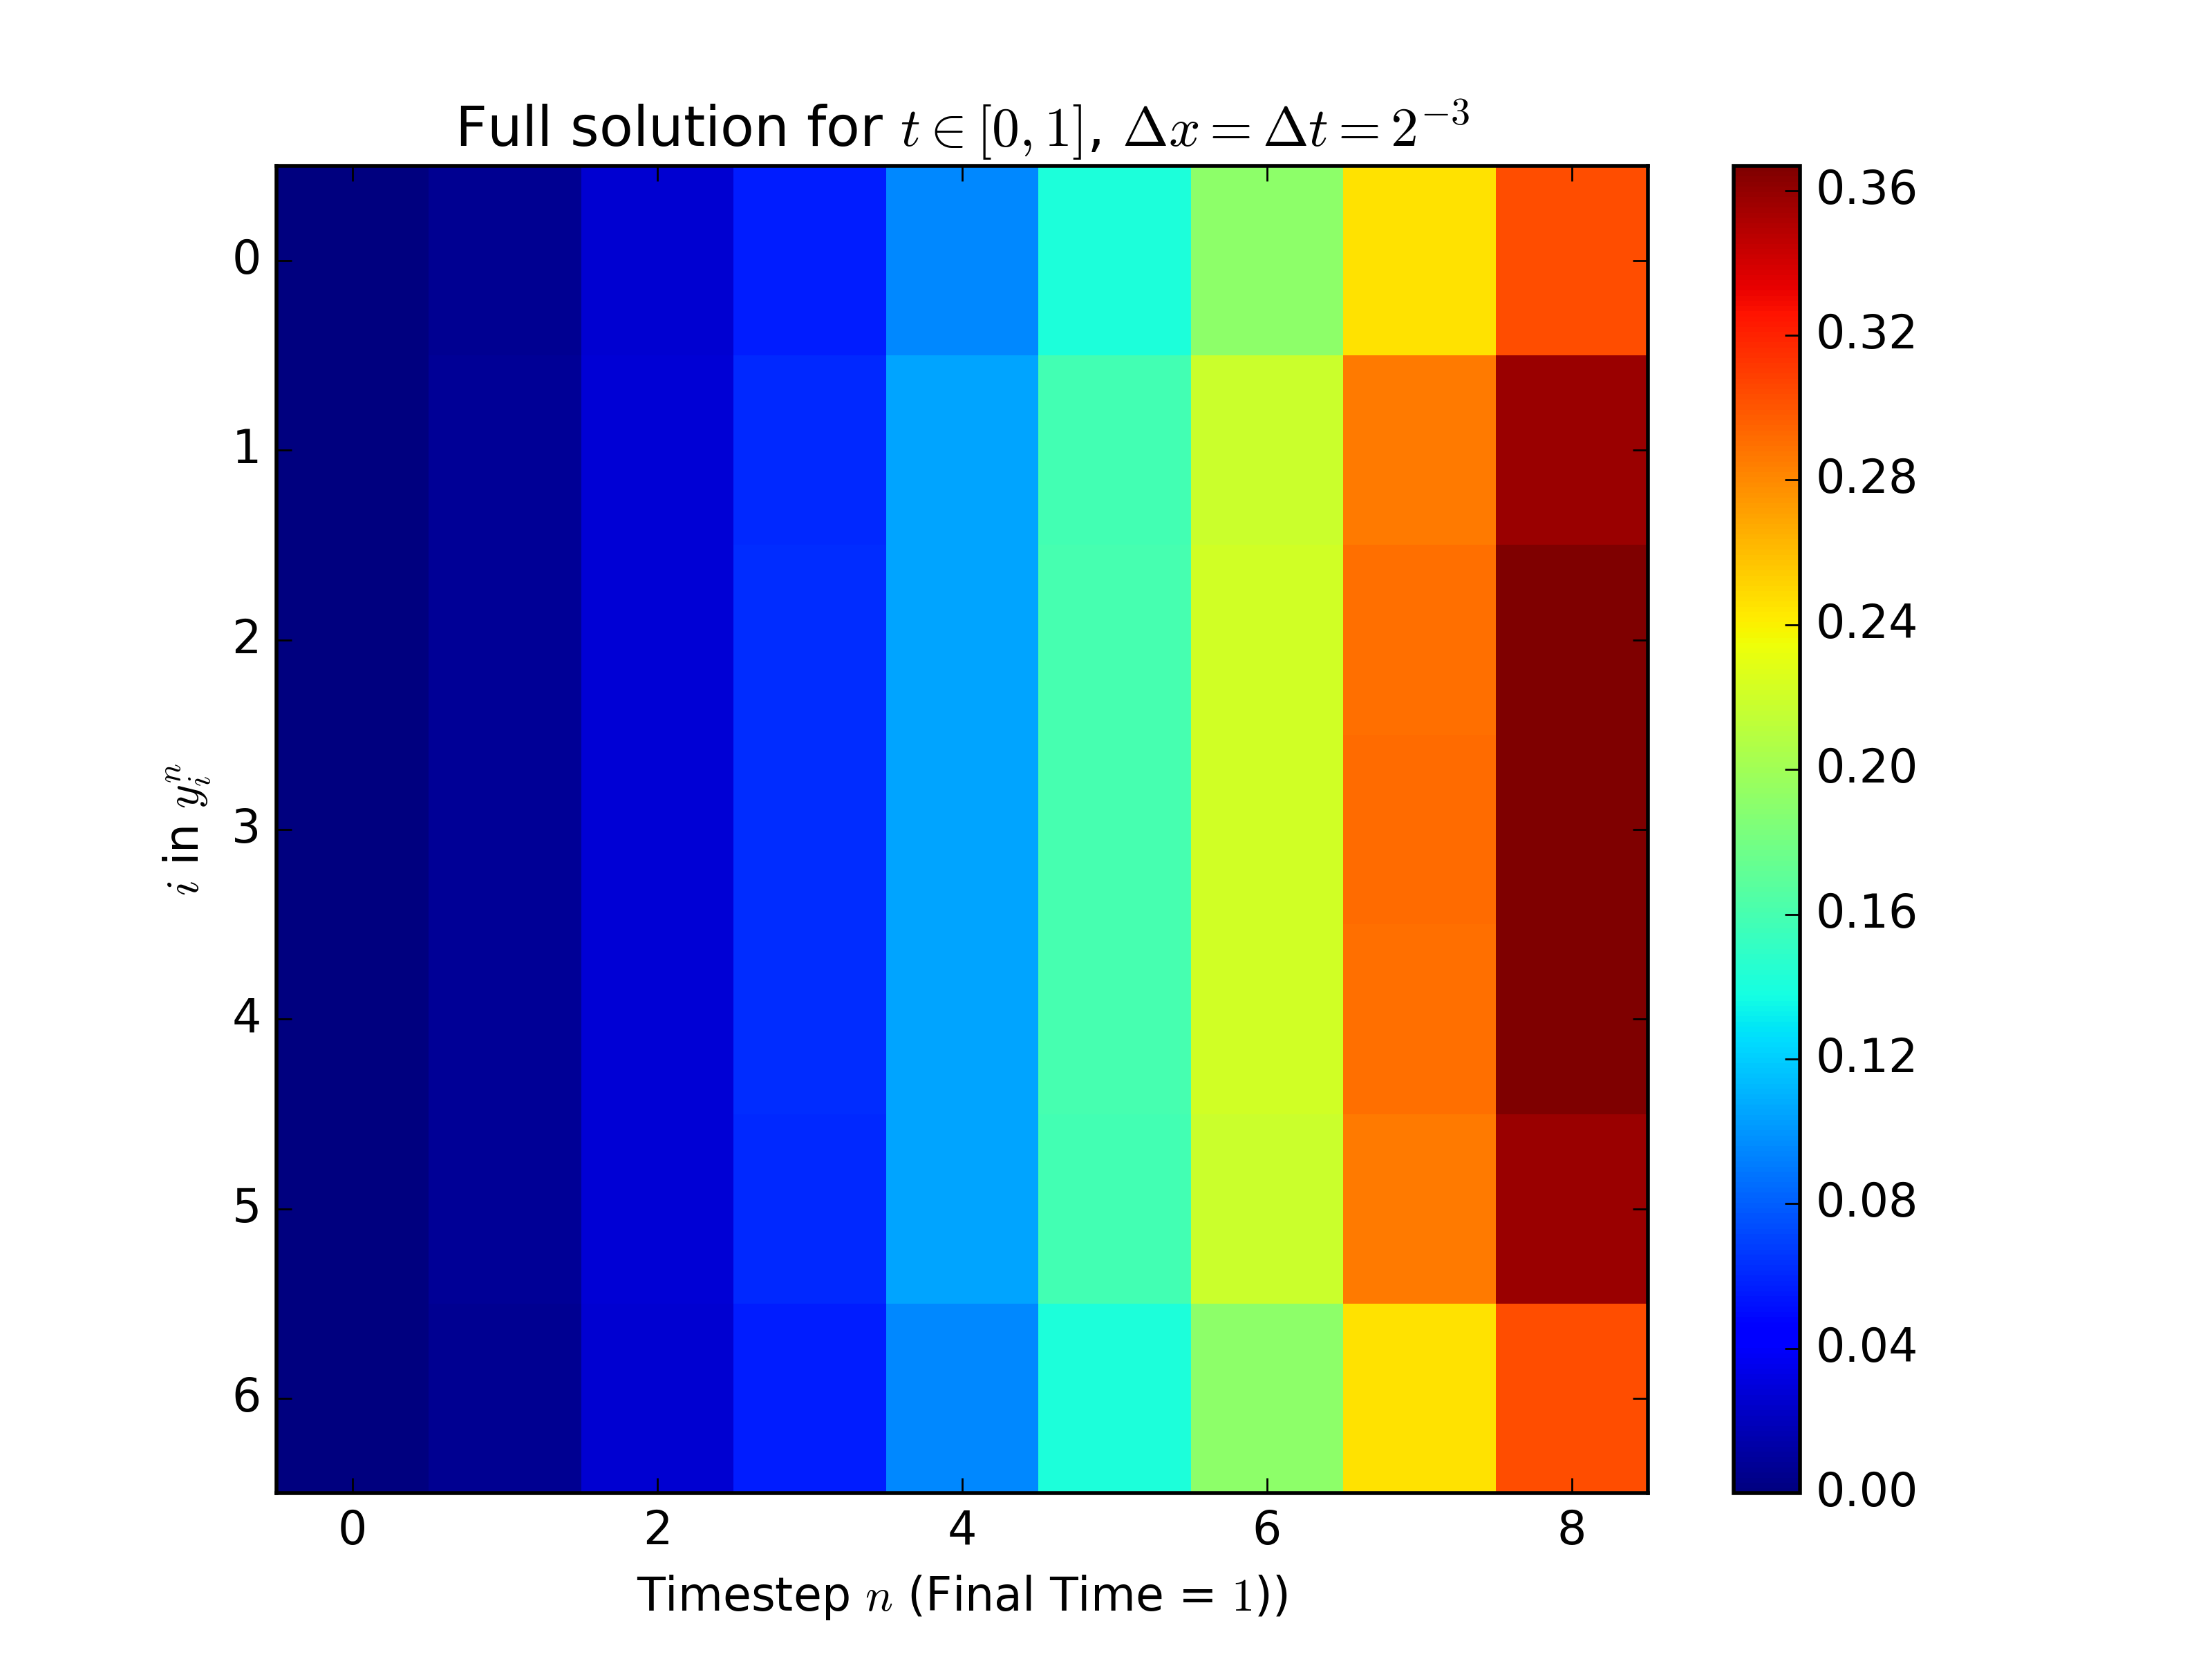
\includegraphics[width=\textwidth]{problem_2_0.png}
\end{minipage}\hfill
\begin{minipage}{0.5\textwidth}
    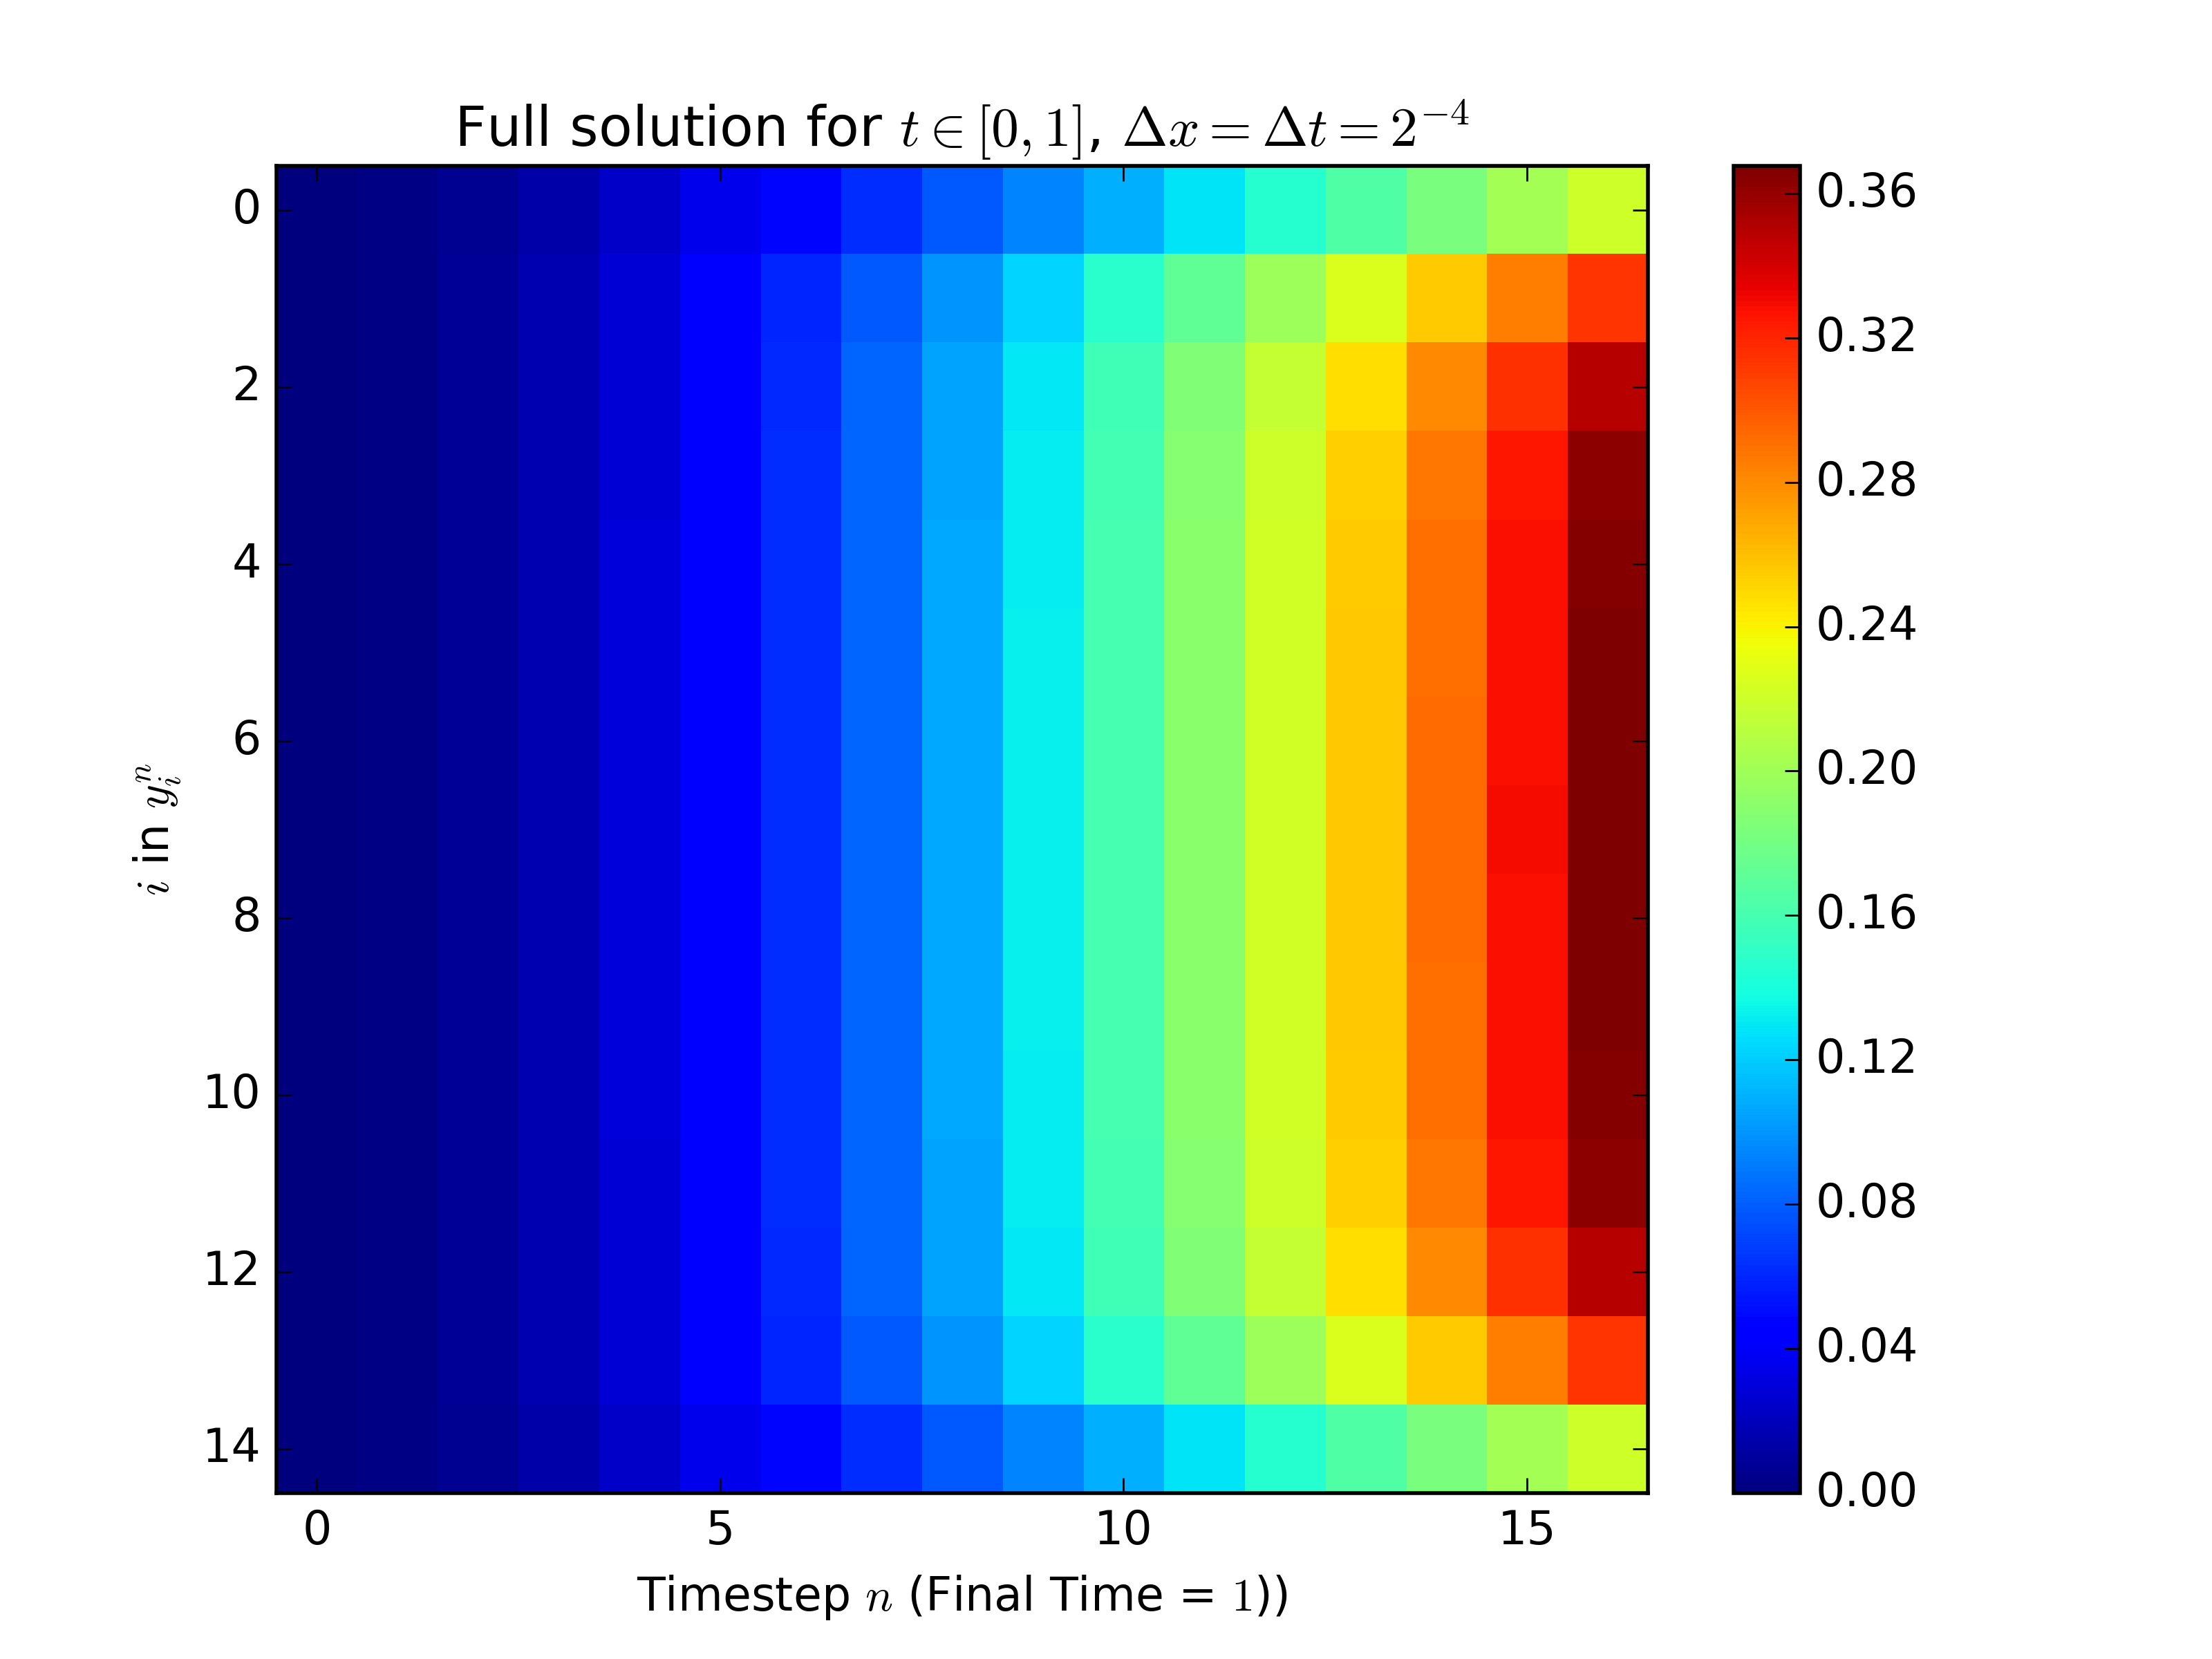
\includegraphics[width=\textwidth]{problem_2_1.png}
\end{minipage}
\begin{minipage}{0.5\textwidth}
    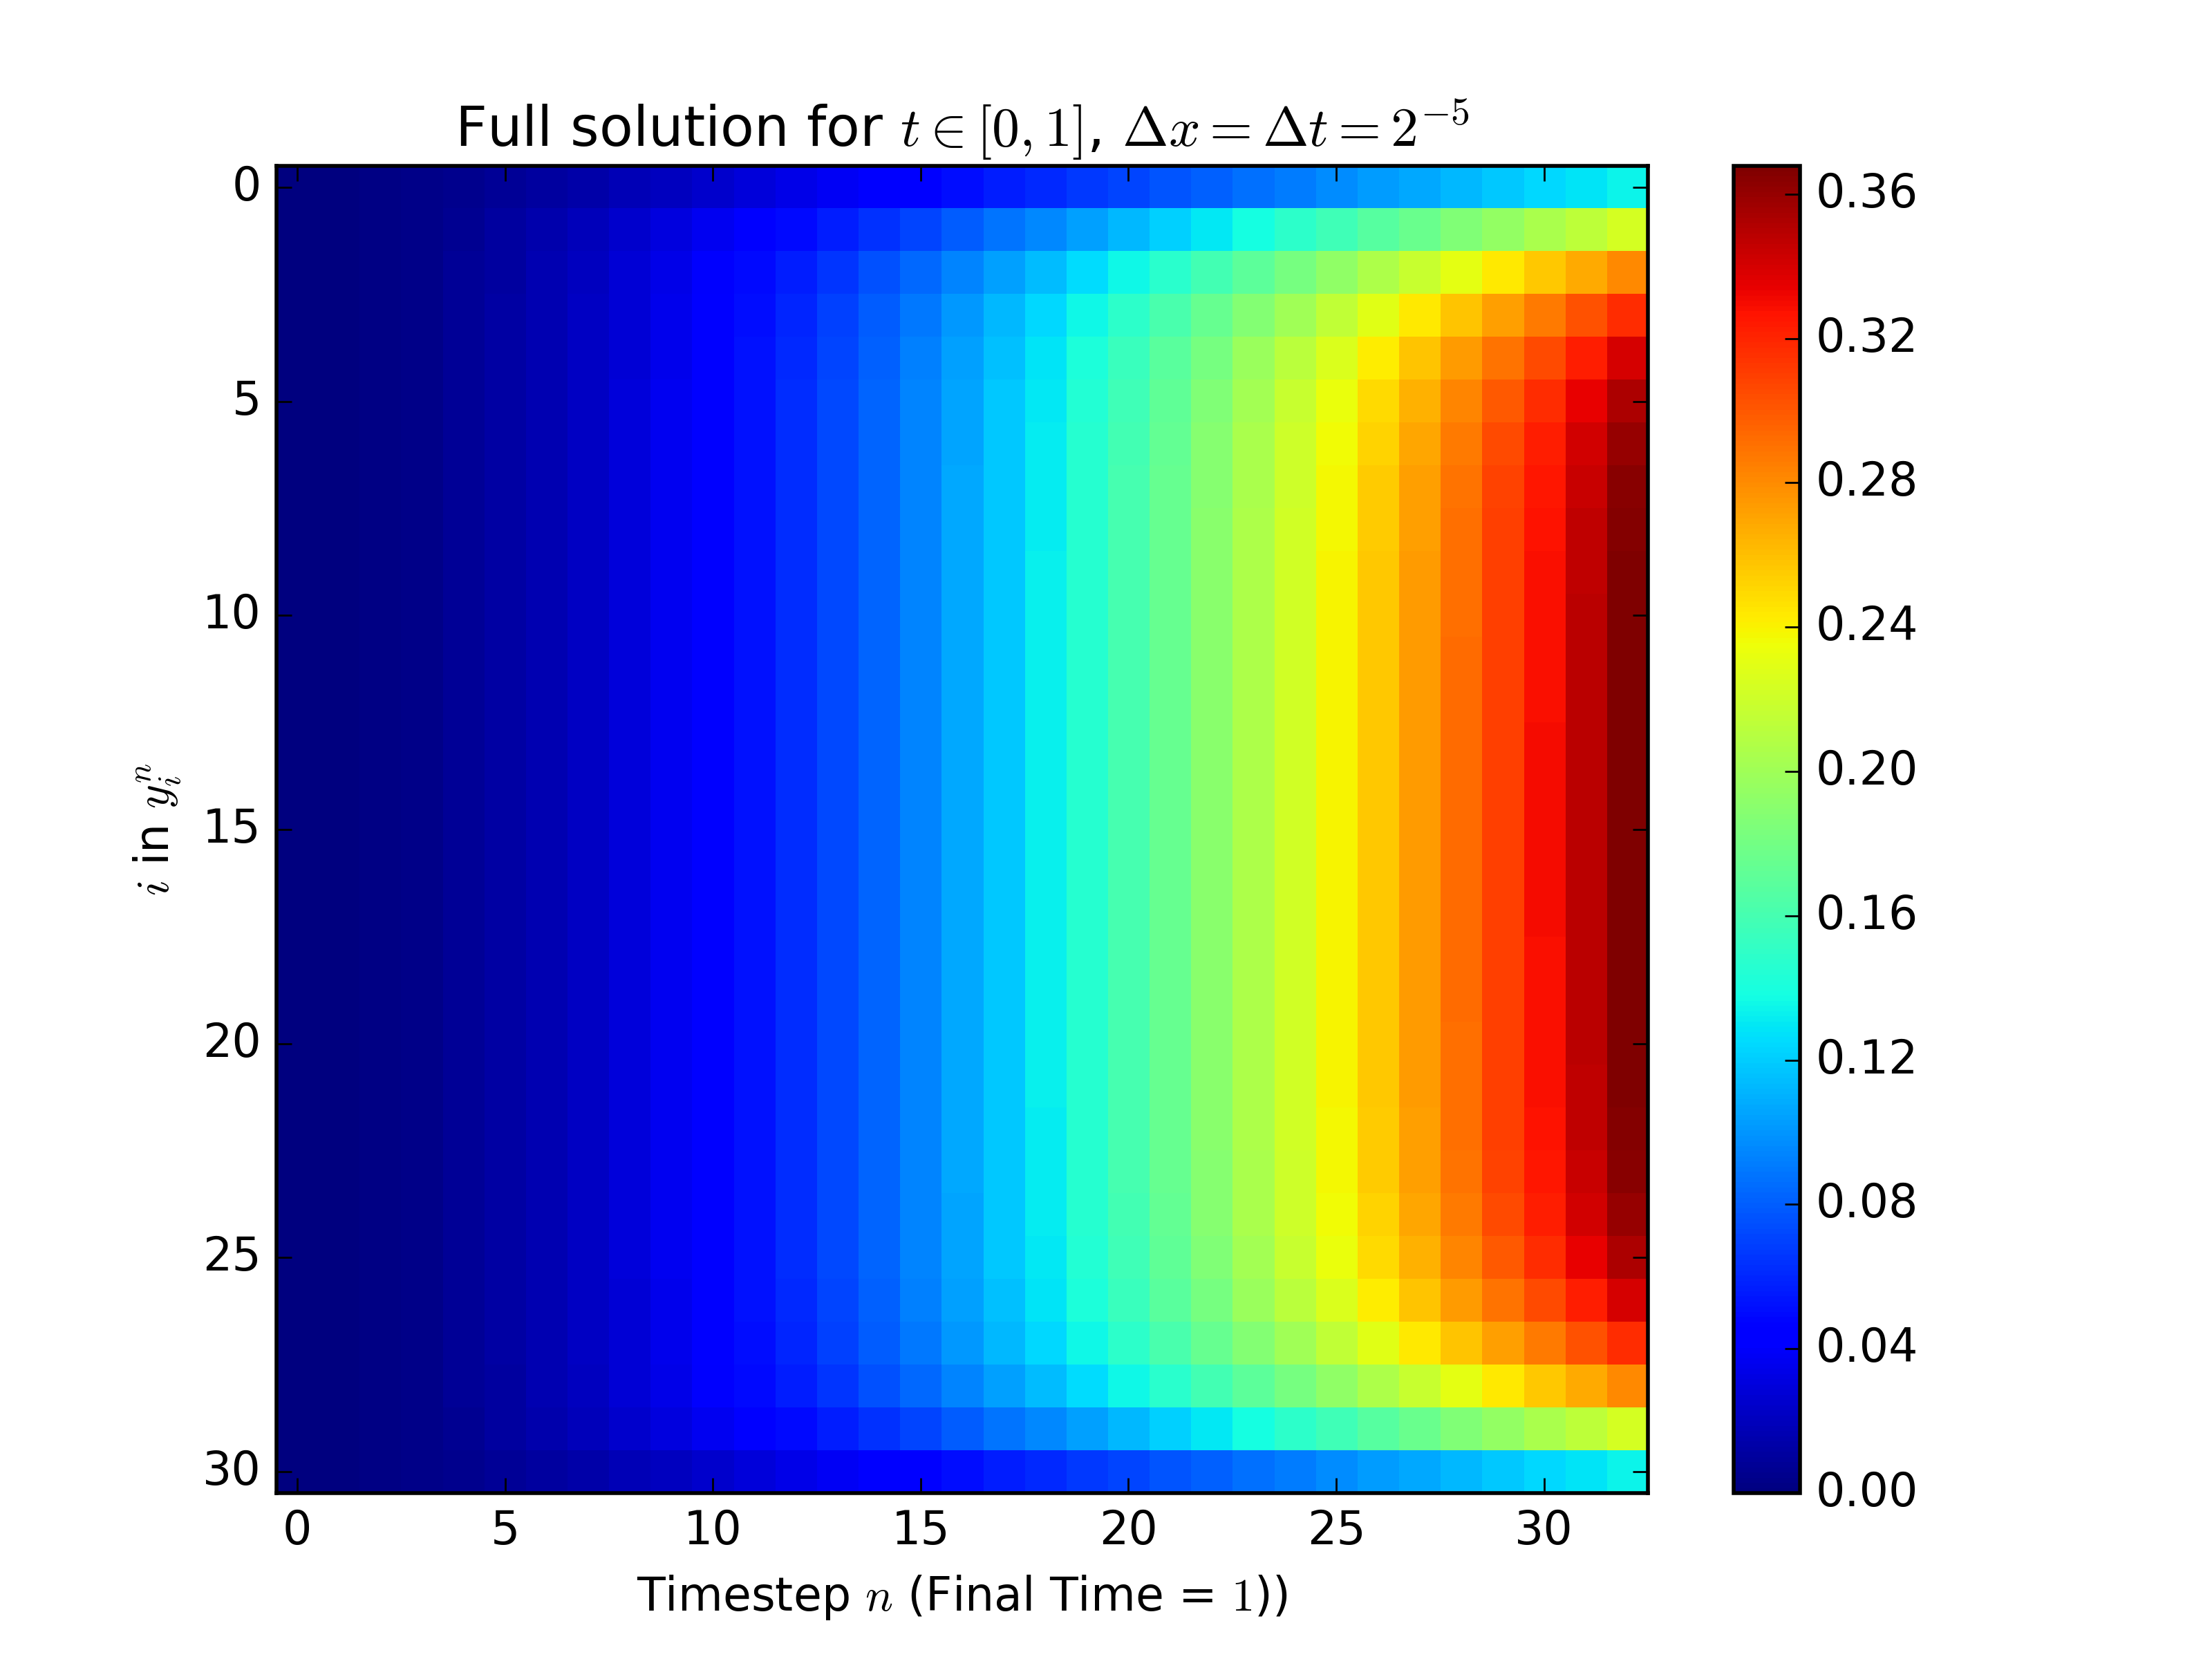
\includegraphics[width=\textwidth]{problem_2_2.png}
\end{minipage}\hfill
\begin{minipage}{0.5\textwidth}
    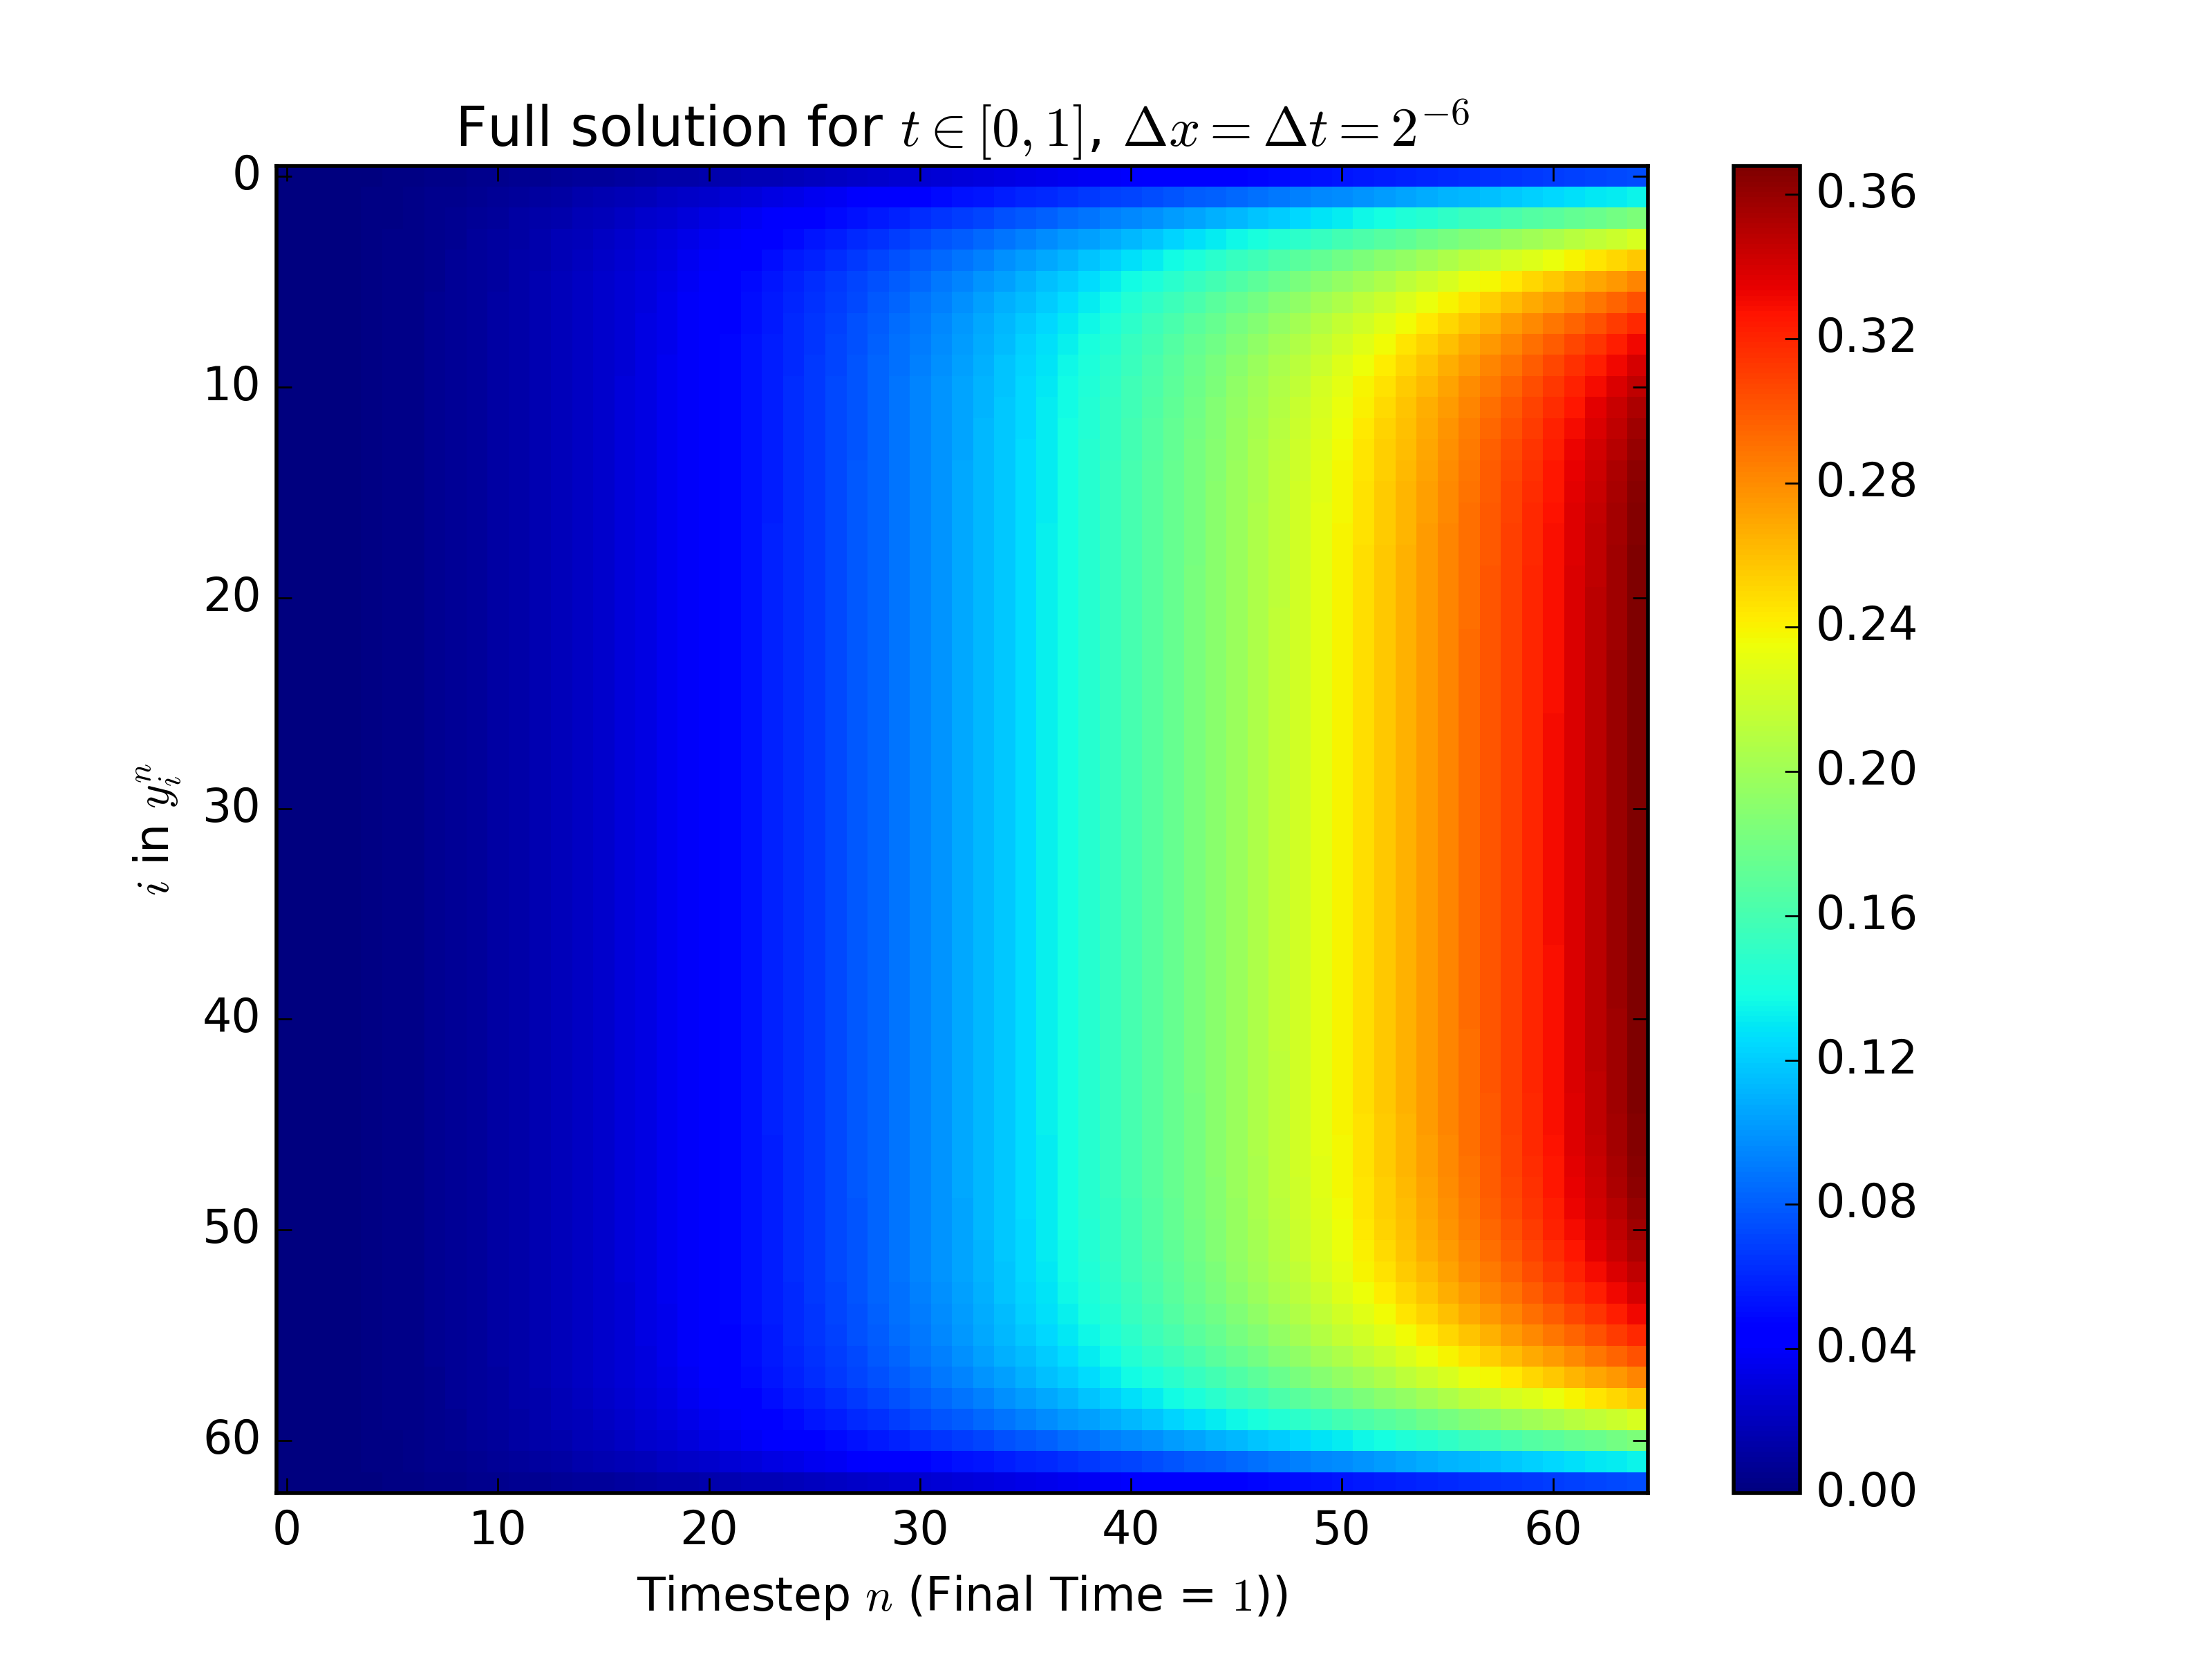
\includegraphics[width=\textwidth]{problem_2_3.png}
\end{minipage}
\begin{minipage}{0.5\textwidth}
    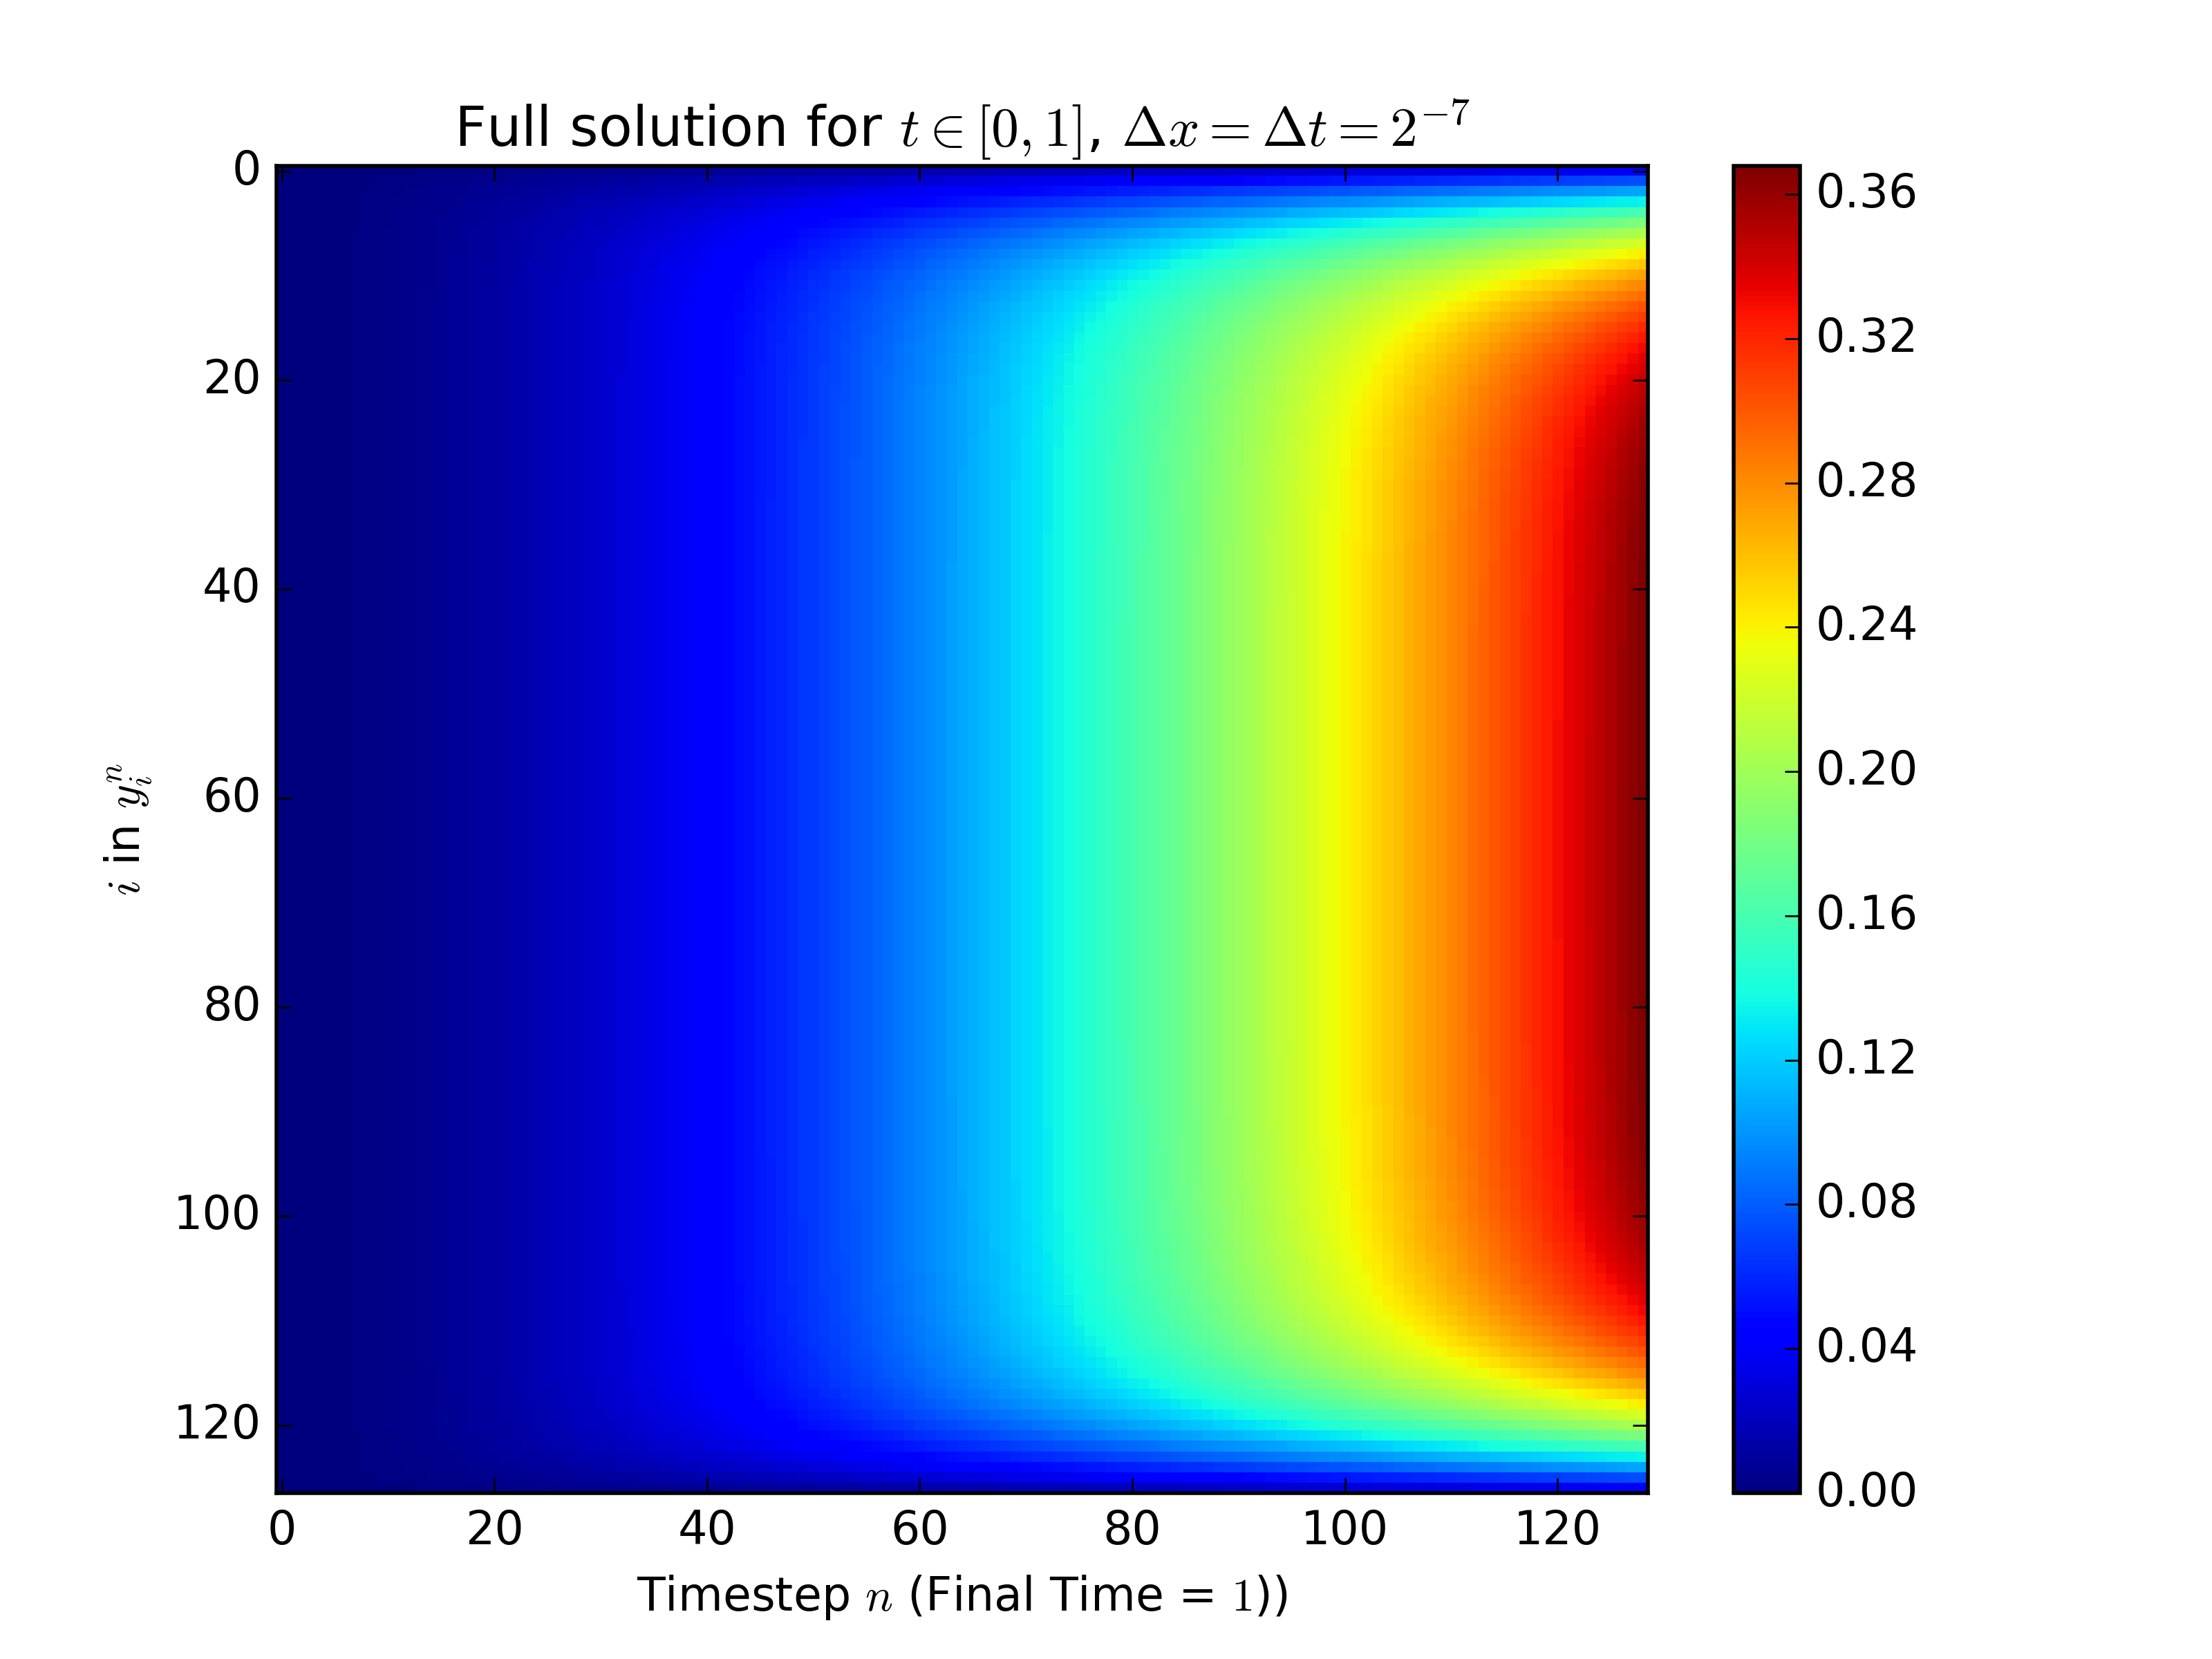
\includegraphics[width=\textwidth]{problem_2_4.png}
\end{minipage}\hfill
\begin{minipage}{0.5\textwidth}
    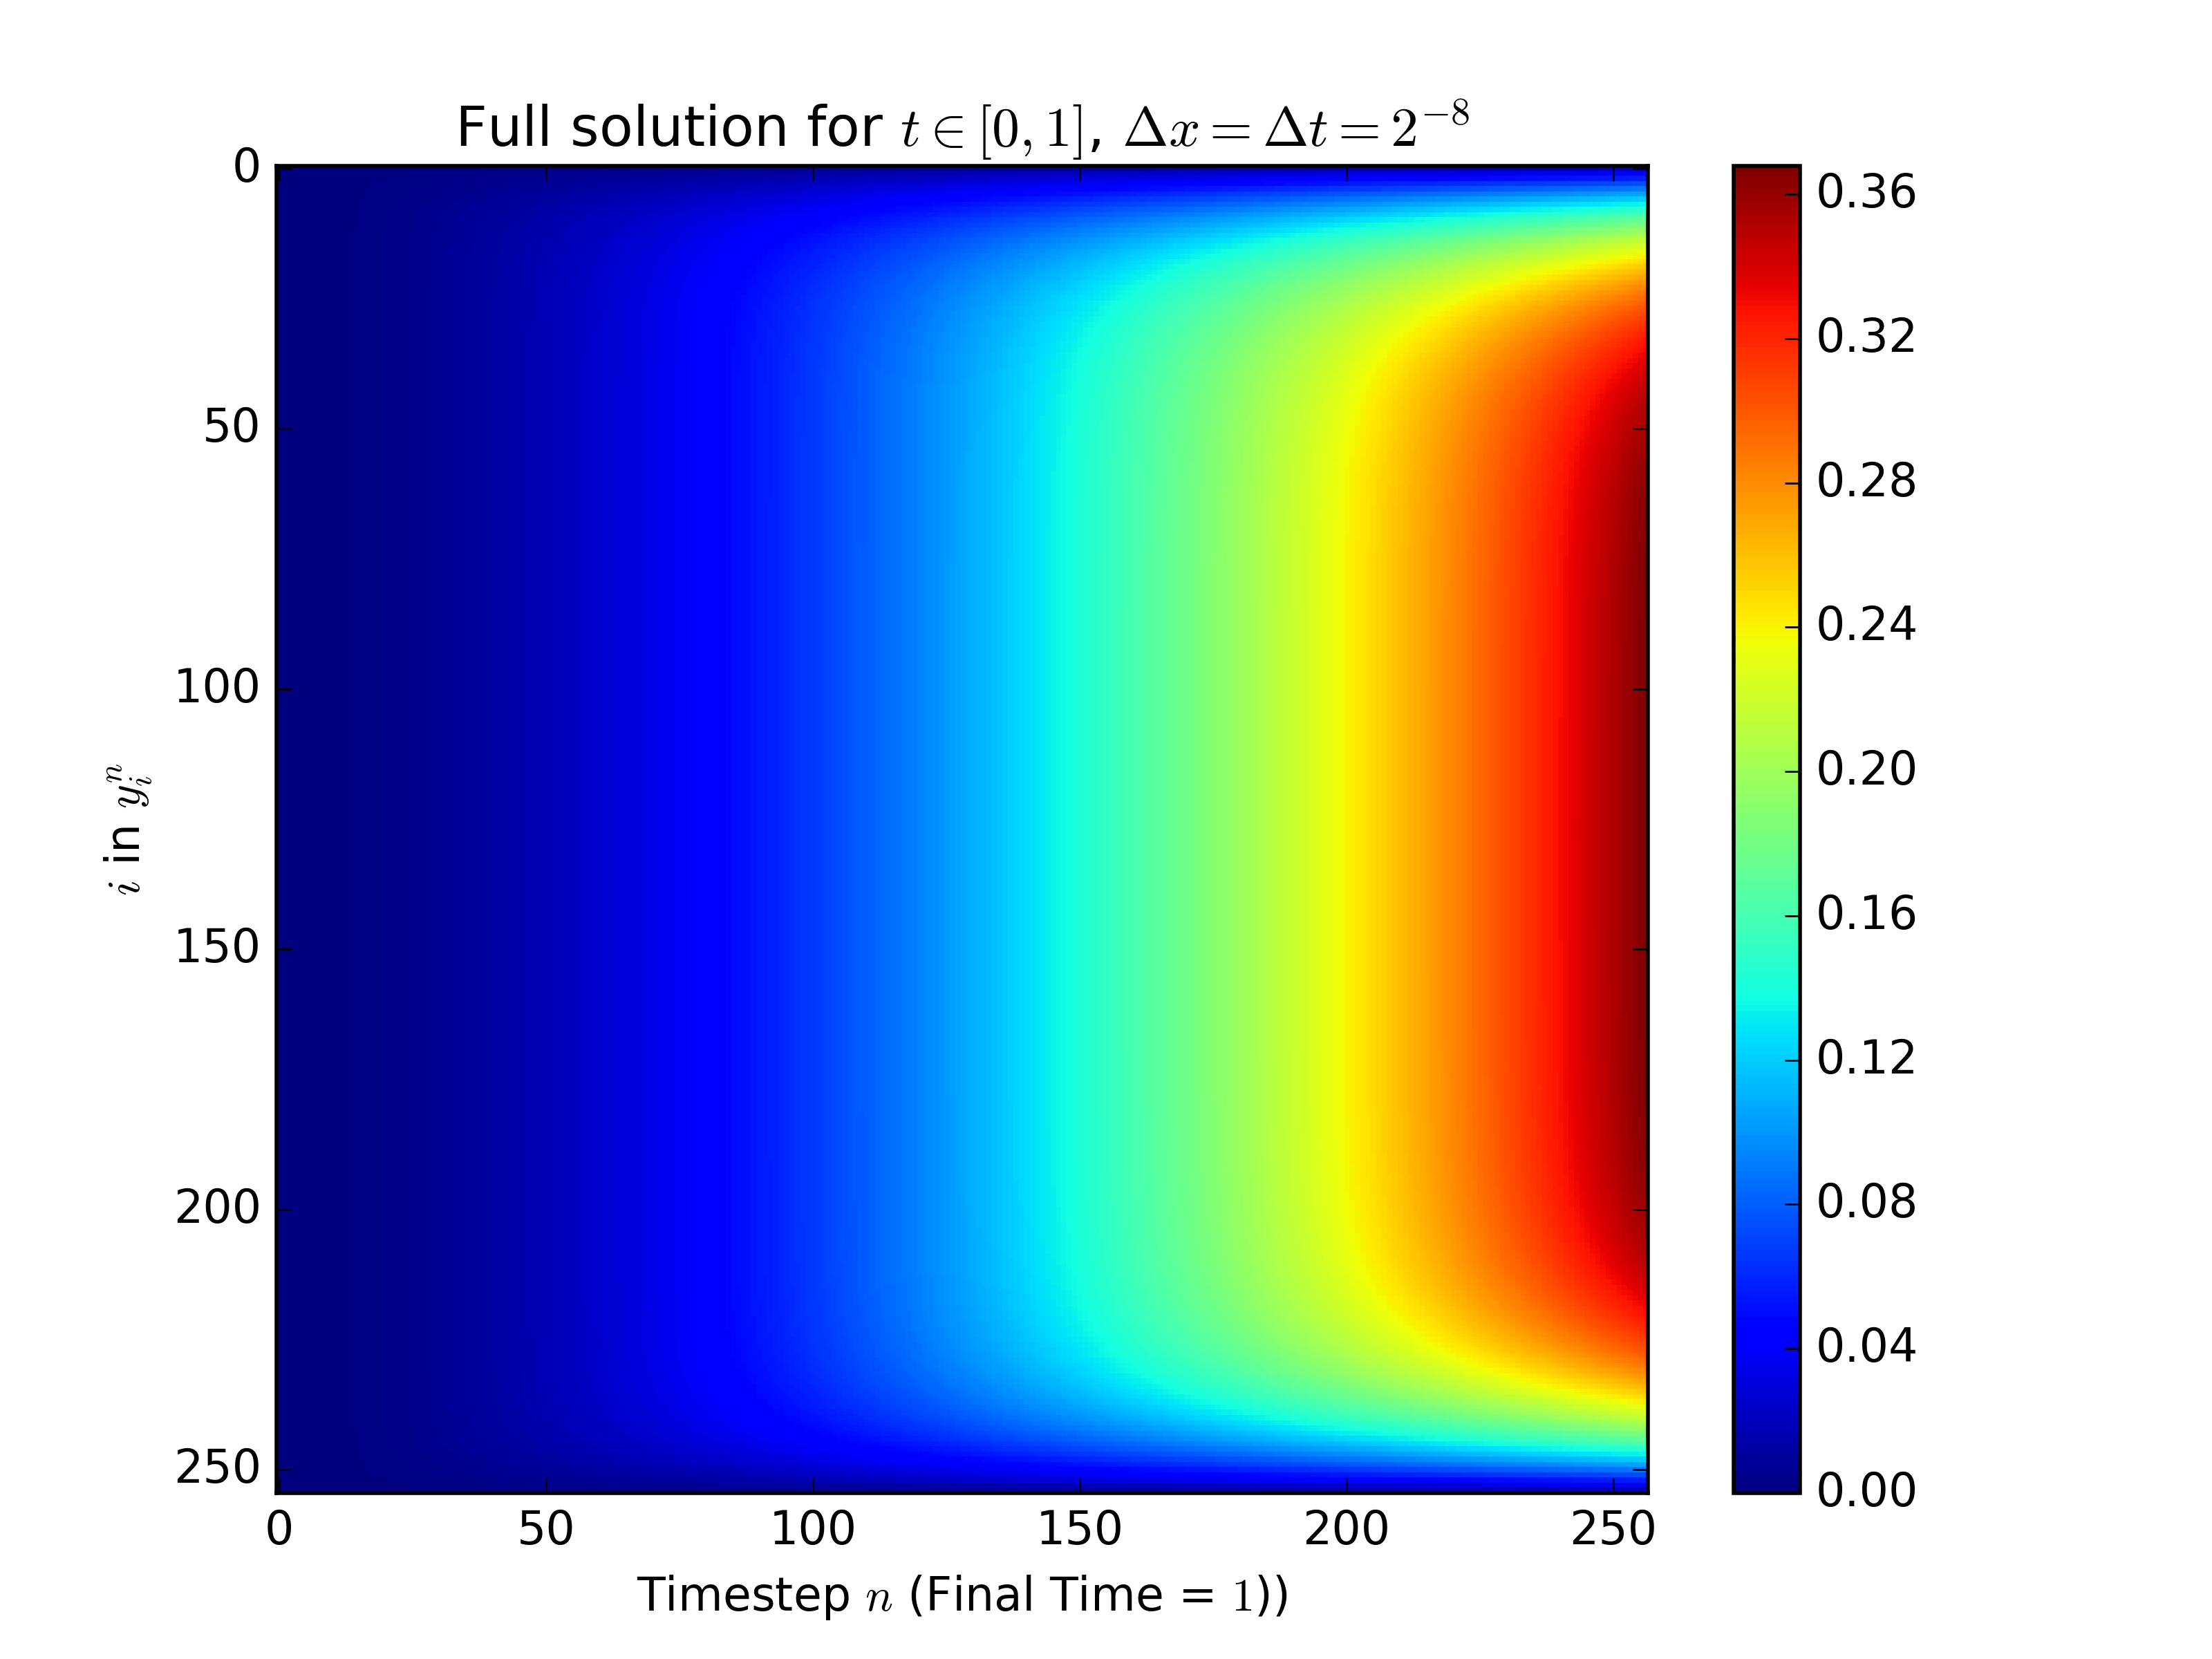
\includegraphics[width=\textwidth]{problem_2_5.png}
\end{minipage}
\begin{minipage}{0.5\textwidth}
    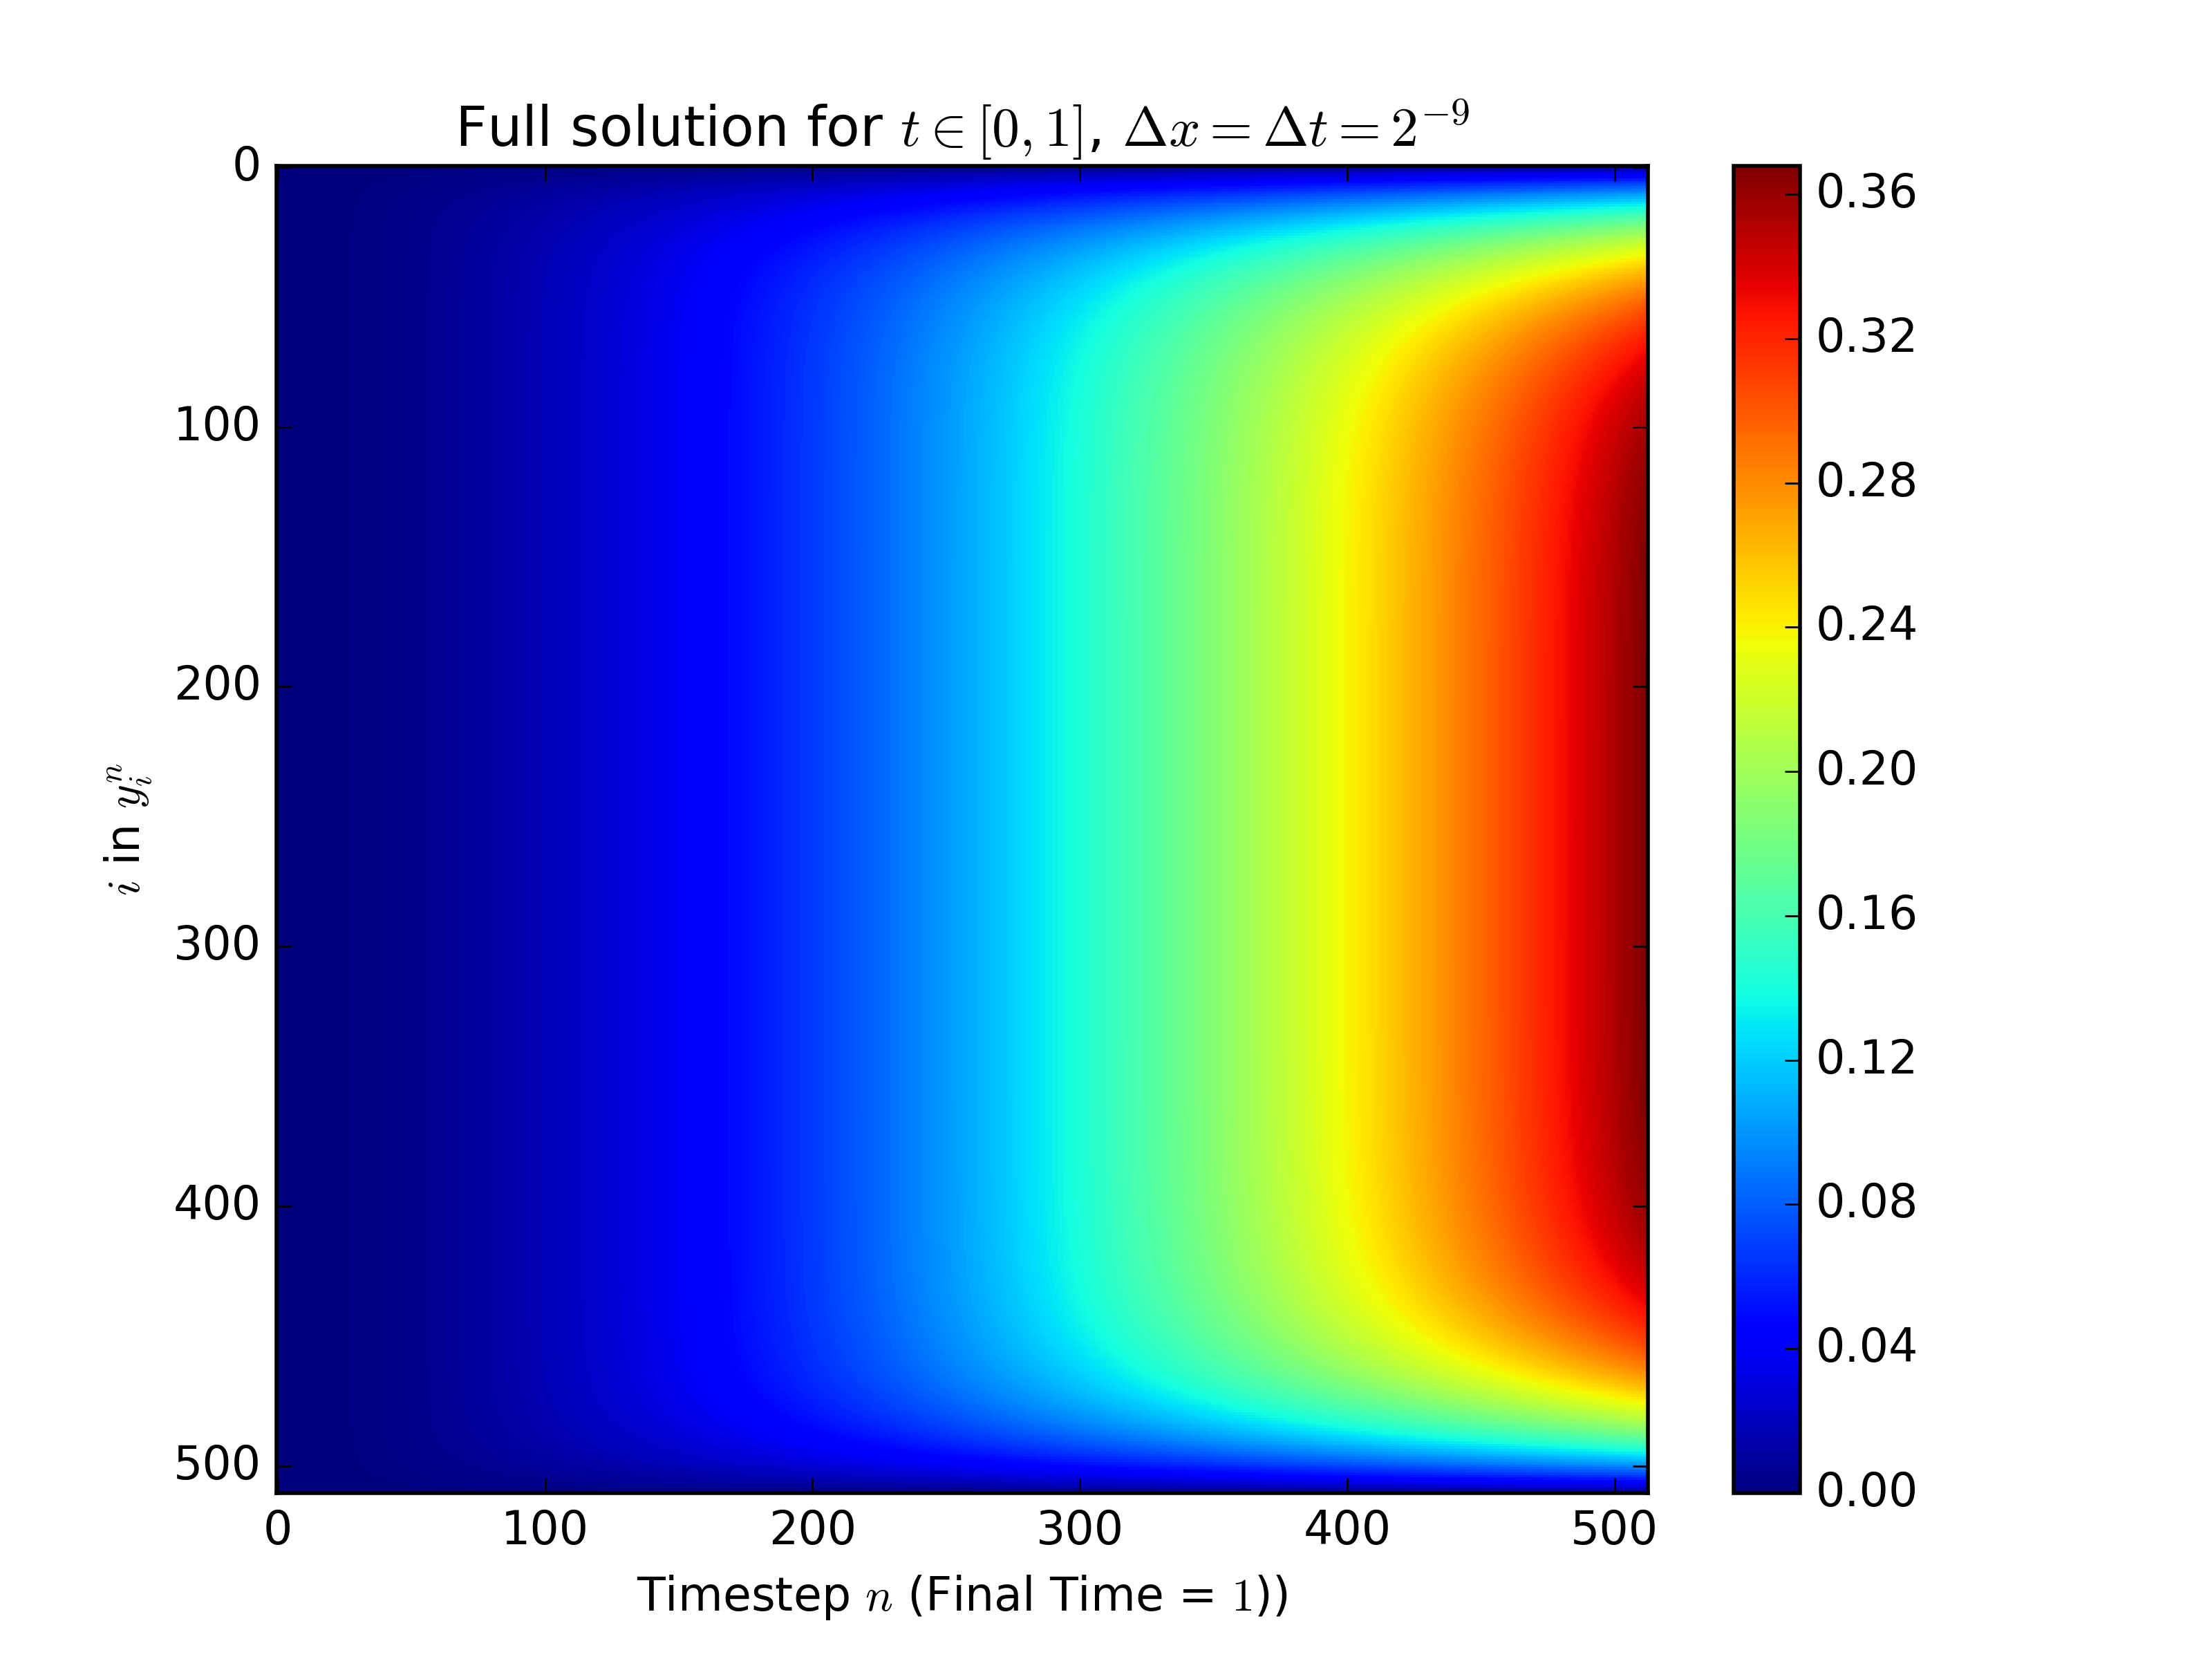
\includegraphics[width=\textwidth]{problem_2_6.png}
\end{minipage}\hfill
\begin{minipage}{0.5\textwidth}
    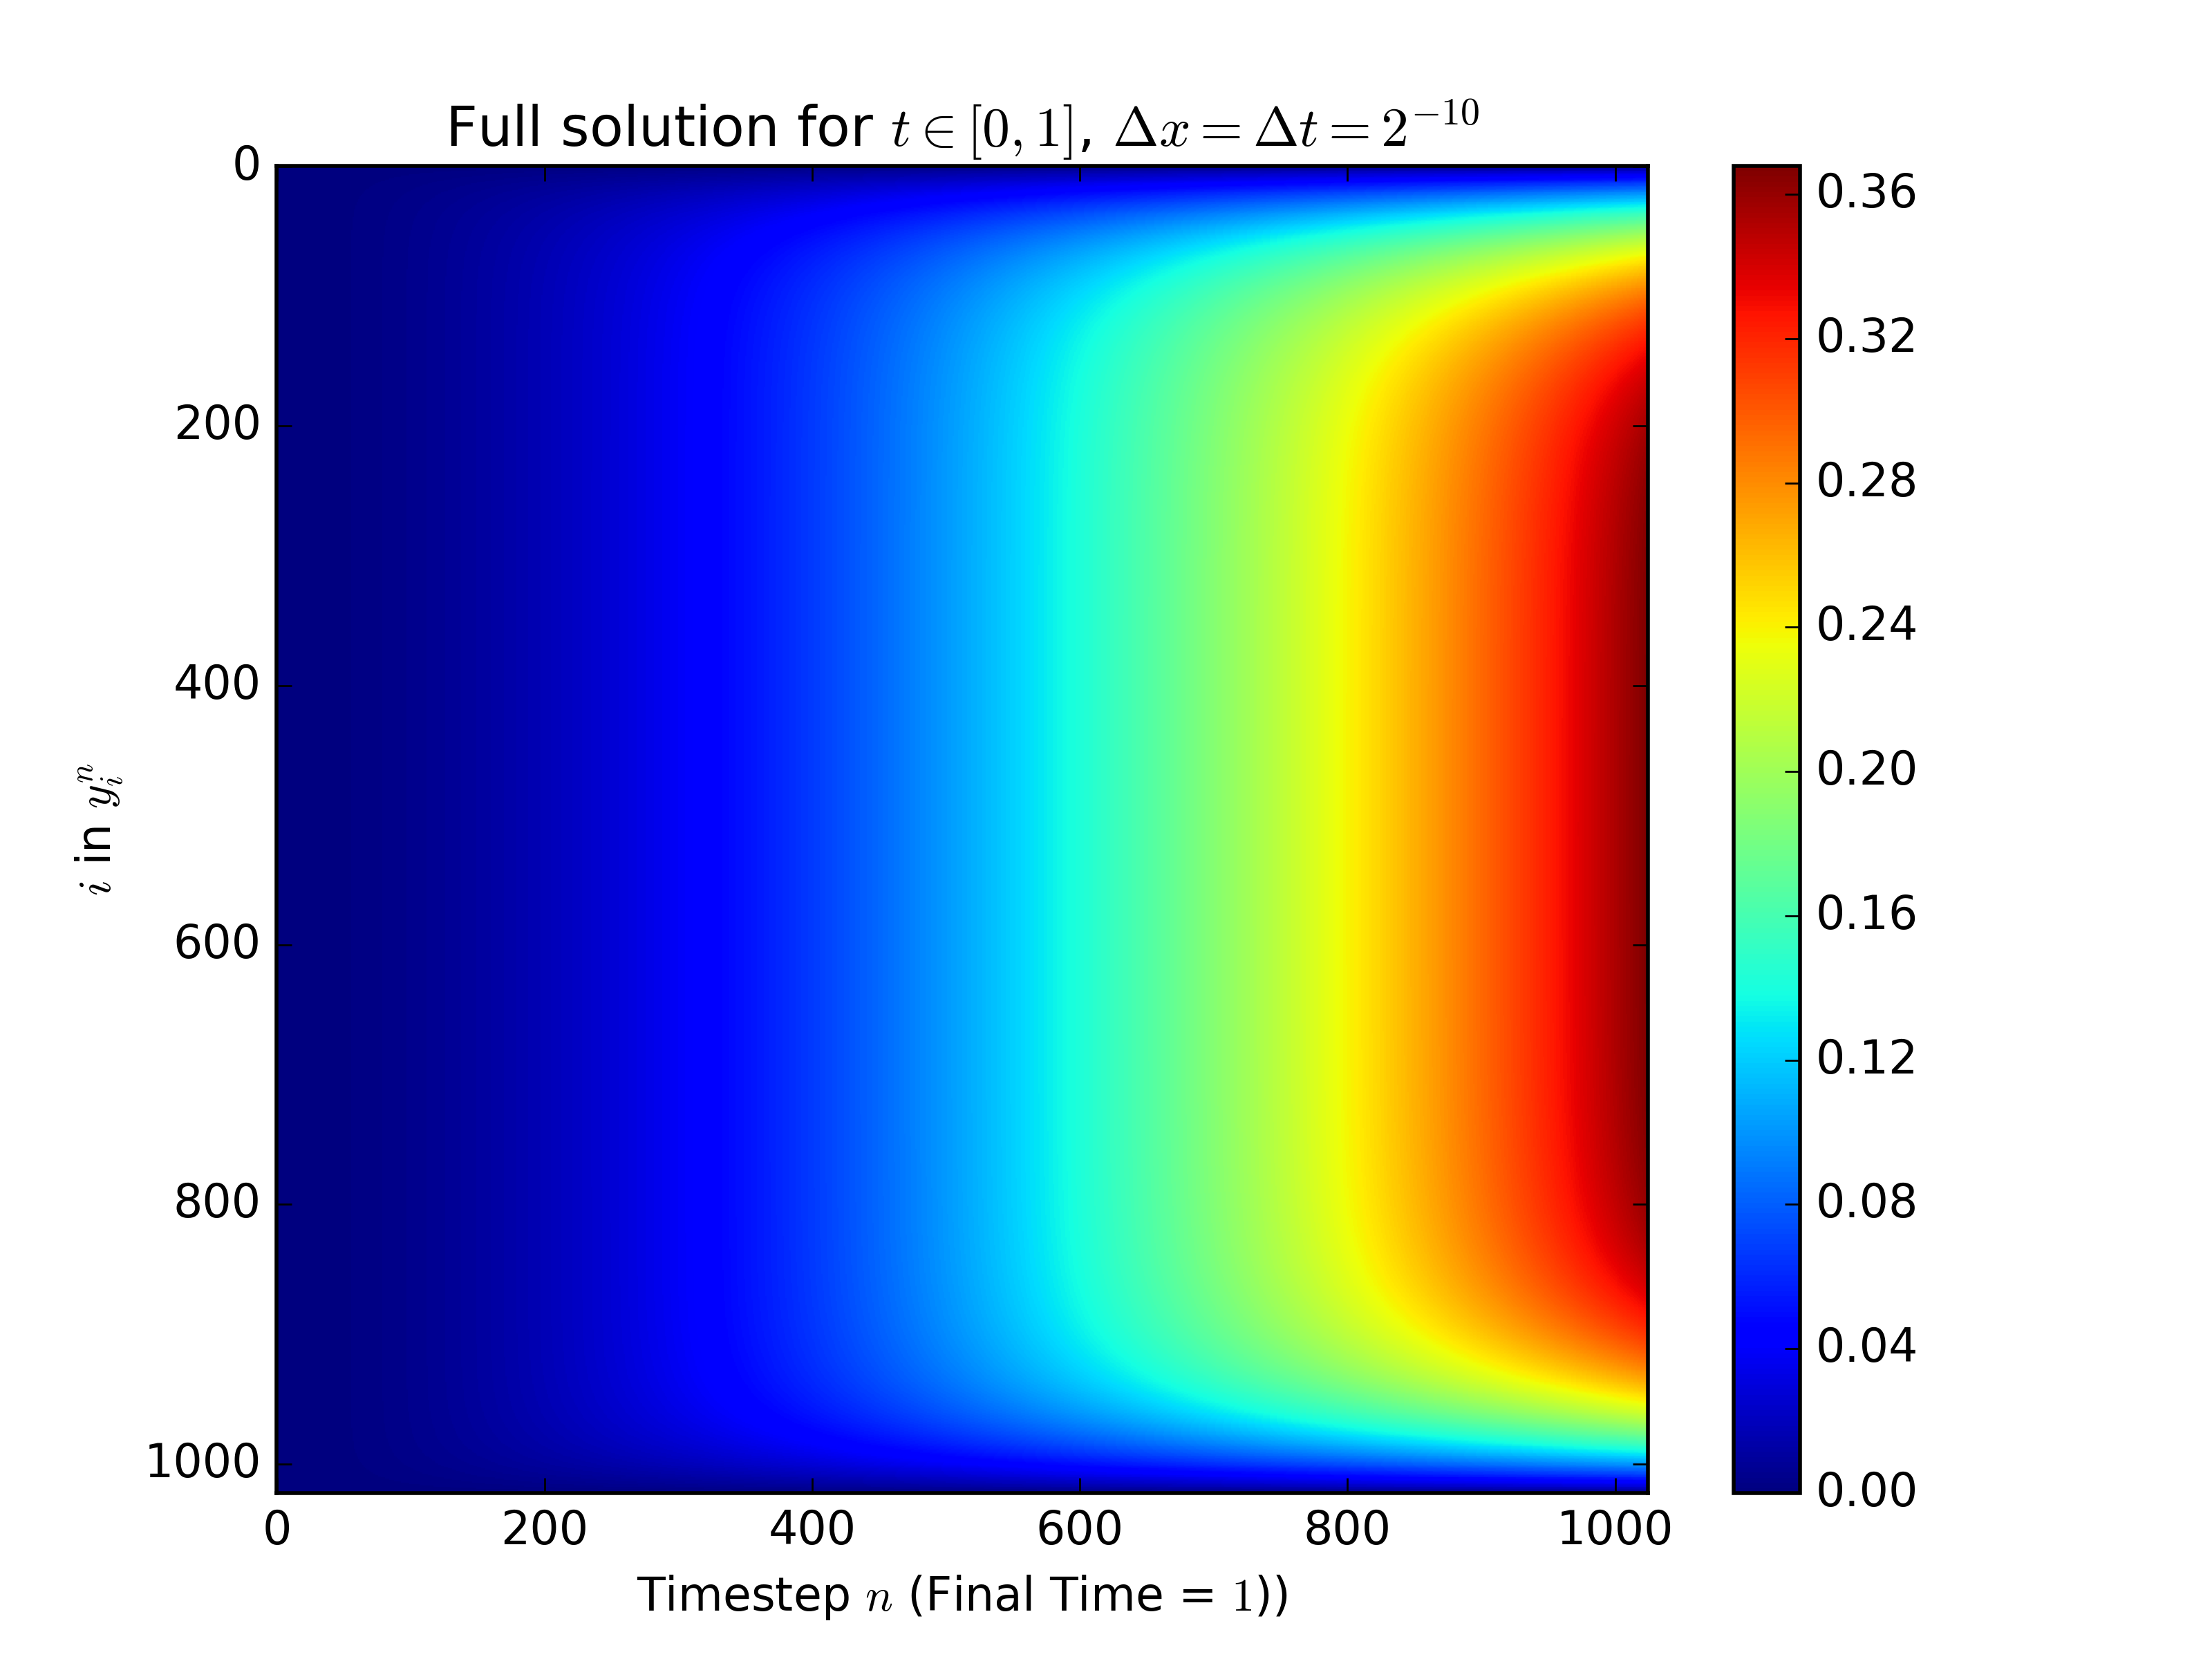
\includegraphics[width=\textwidth]{problem_2_7.png}
\end{minipage}
Clearly even large $\Dx$ and $\Dt$ do a reasonable job at approximating the system at very small $\Dx$ and $\Dt$.  To compare successive errors, define a restriction operator $R$ so that $u_{\Dx,\text{coarse}} = Ru_{\Dx,\text{fine}}$ where $(u_{\Dx,\text{coarse}})_i = \qty(u_{\Dx,\text{fine}})_{2i+1}$.  In other words, the restriction operator simply takes the values at successive corresponding positions.  Then use the discrete $\norm{\cdot}_1$ to calculate $\norm{u_{2\Dx,\text{fine}} - u_{\Dx,\text{coarse}}}_1$.  Finally, calculate this value for each pair of successive simulations (halving $\Dx$ and $\Dt$ in each step) and compute the ratios, which gives the following results:
\begin{align*}
    \begin{array}{||c|c||}\hline\hline
        \vphantom{\frac{\dfrac{1}{1}}{\dfrac{1}{1}}}\frac{\norm{u_{2\Dx,\text{fine}} - u_{\Dx,\text{coarse}}}_1}{\norm{u_{\Dx,\text{fine}} - u_{\nicefrac{\Dx}{2},\text{coarse}}}_1} & \text{Ratio} \\\hline\hline
        \vphantom{\frac{\dfrac{1}{1}}{\dfrac{1}{1}}}\frac{\norm{u_{2^{-3},\text{fine}} - u_{2^{-4},\text{coarse}}}_1}{\norm{u_{2^{-4},\text{fine}} - u_{2^{-5},\text{coarse}}}_1} & 3.12909673006 \\\hline
        \vphantom{\frac{\dfrac{1}{1}}{\dfrac{1}{1}}}\frac{\norm{u_{2^{-4},\text{fine}} - u_{2^{-5},\text{coarse}}}_1}{\norm{u_{2^{-5},\text{fine}} - u_{2^{-6},\text{coarse}}}_1} & 3.78137533007 \\\hline
        \vphantom{\frac{\dfrac{1}{1}}{\dfrac{1}{1}}}\frac{\norm{u_{2^{-5},\text{fine}} - u_{2^{-6},\text{coarse}}}_1}{\norm{u_{2^{-6},\text{fine}} - u_{2^{-7},\text{coarse}}}_1} & 3.94618495735 \\\hline
        \vphantom{\frac{\dfrac{1}{1}}{\dfrac{1}{1}}}\frac{\norm{u_{2^{-6},\text{fine}} - u_{2^{-7},\text{coarse}}}_1}{\norm{u_{2^{-7},\text{fine}} - u_{2^{-8},\text{coarse}}}_1} & 3.98660432714 \\\hline
        \vphantom{\frac{\dfrac{1}{1}}{\dfrac{1}{1}}}\frac{\norm{u_{2^{-7},\text{fine}} - u_{2^{-8},\text{coarse}}}_1}{\norm{u_{2^{-8},\text{fine}} - u_{2^{-9},\text{coarse}}}_1} & 3.99665475958 \\\hline
        \vphantom{\frac{\dfrac{1}{1}}{\dfrac{1}{1}}}\frac{\norm{u_{2^{-8},\text{fine}} - u_{2^{-9},\text{coarse}}}_1}{\norm{u_{2^{-9},\text{fine}} - u_{2^{-10},\text{coarse}}}_1} & 3.99916427638 \\\hline\hline
    \end{array}
\end{align*}
The successive ratios are clearly approaching $4$, which shows evidence the method is second-order accurate in both time and space.







\pagebreak
\problem{Problem 3}{
\begin{gather*}
    u_t = u_{xx}, \qquad 0 < x < 1\\
    u(0,t) = 1, \qquad u(1,t) = 0\\
    u(x,0) = \begin{cases}
        1 & \text{ if } x < 0.5\\
        0 & \text{ if } x \geq 0.5
    \end{cases}
\end{gather*}
\begin{enumerate}[\ \ (a)]
    \item Use Crank-Nicolson with grid spacing $\Delta x = 0.02$ and time step $0.1$ to solve the problem up to time $t = 1$.  Comment on your results.  What is wrong with this solution?
    \item Give a mathematical argument to explain the unphysical behavior you observed in the numerical solution.
    \item Repeat the simulation using BDF2, and discuss why the unphysical behavior is not present in the numerical solution for any time step.
\end{enumerate}}

\begin{enumerate}[\ \ (a)]
    \item Here is the solution to the above system for $t = 0$ to $t = 1$.

    \begin{minipage}{\textwidth}
        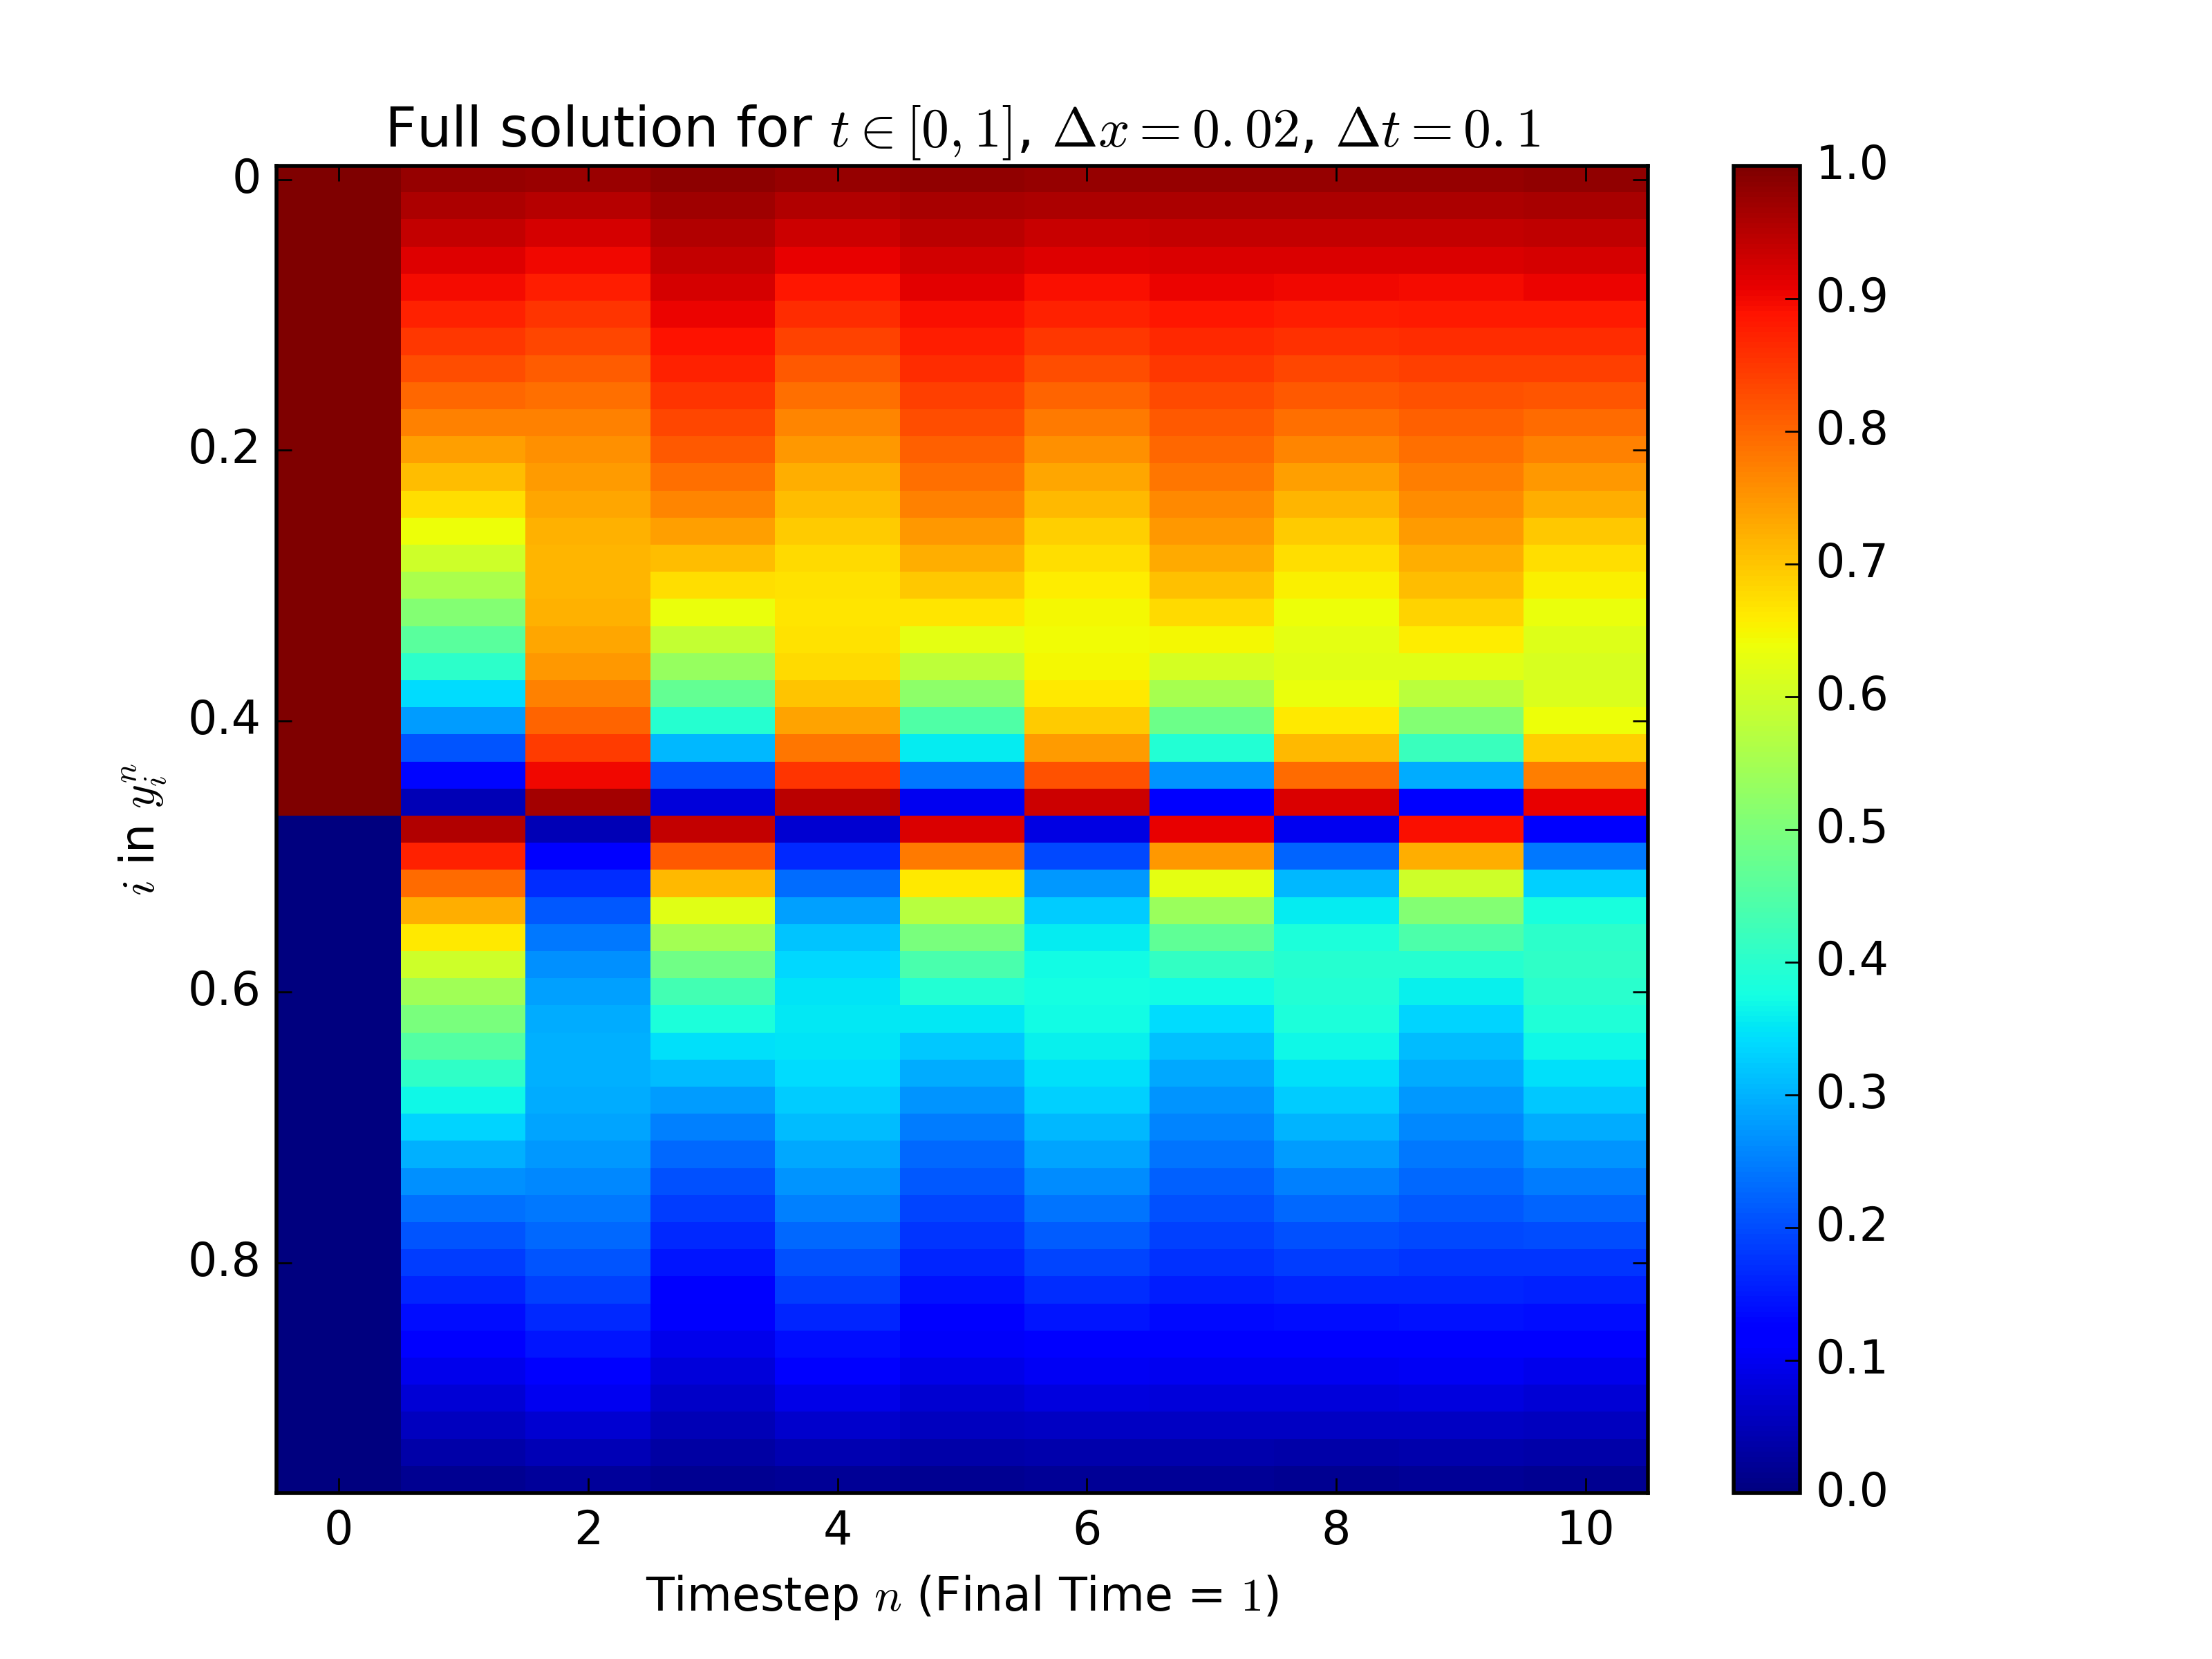
\includegraphics[width=\textwidth]{problem_3a.png}
    \end{minipage}
    This is clearly unphysical, espencially near the initial discontinuity $x \approx 0.5$.  The timestep is too large in relation to the diffusion coefficient and spacestep.  The following show simulations where either $D$ or $\Dt$ are significantly decreased:

    \begin{minipage}{0.5\textwidth}
        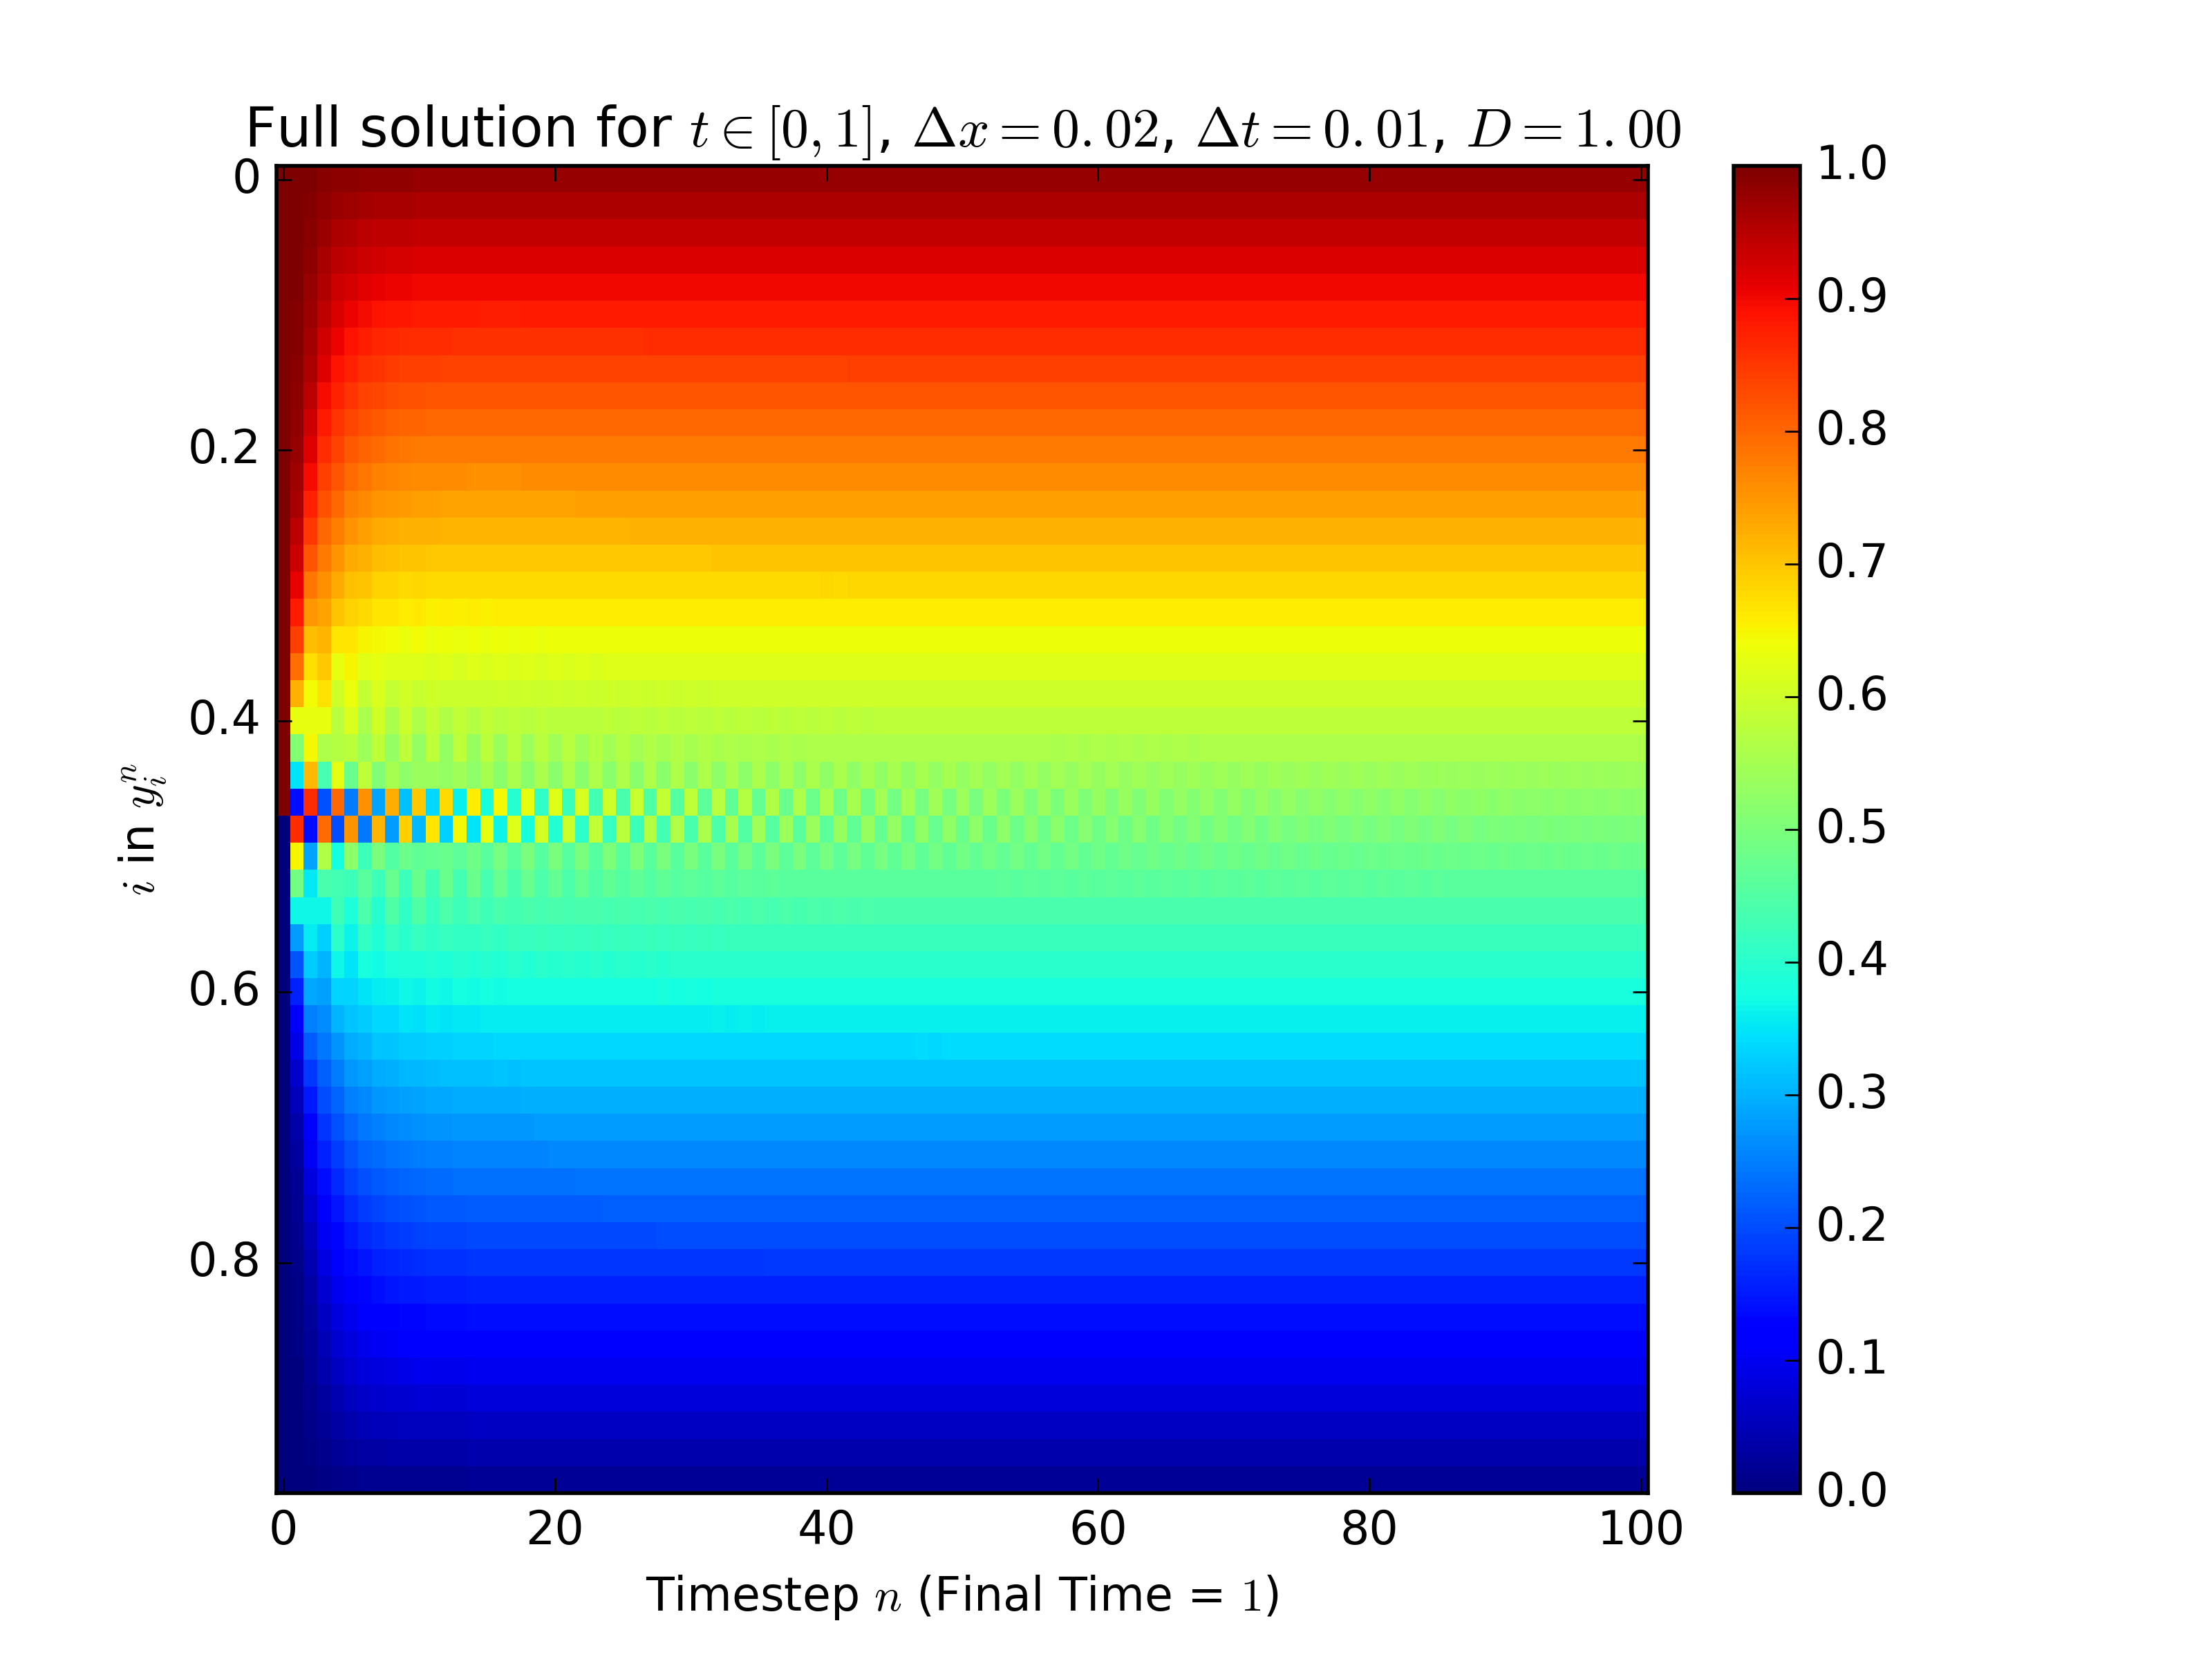
\includegraphics[width=\textwidth]{problem_3a_a.png}
    \end{minipage}\hfill
    \begin{minipage}{0.5\textwidth}
        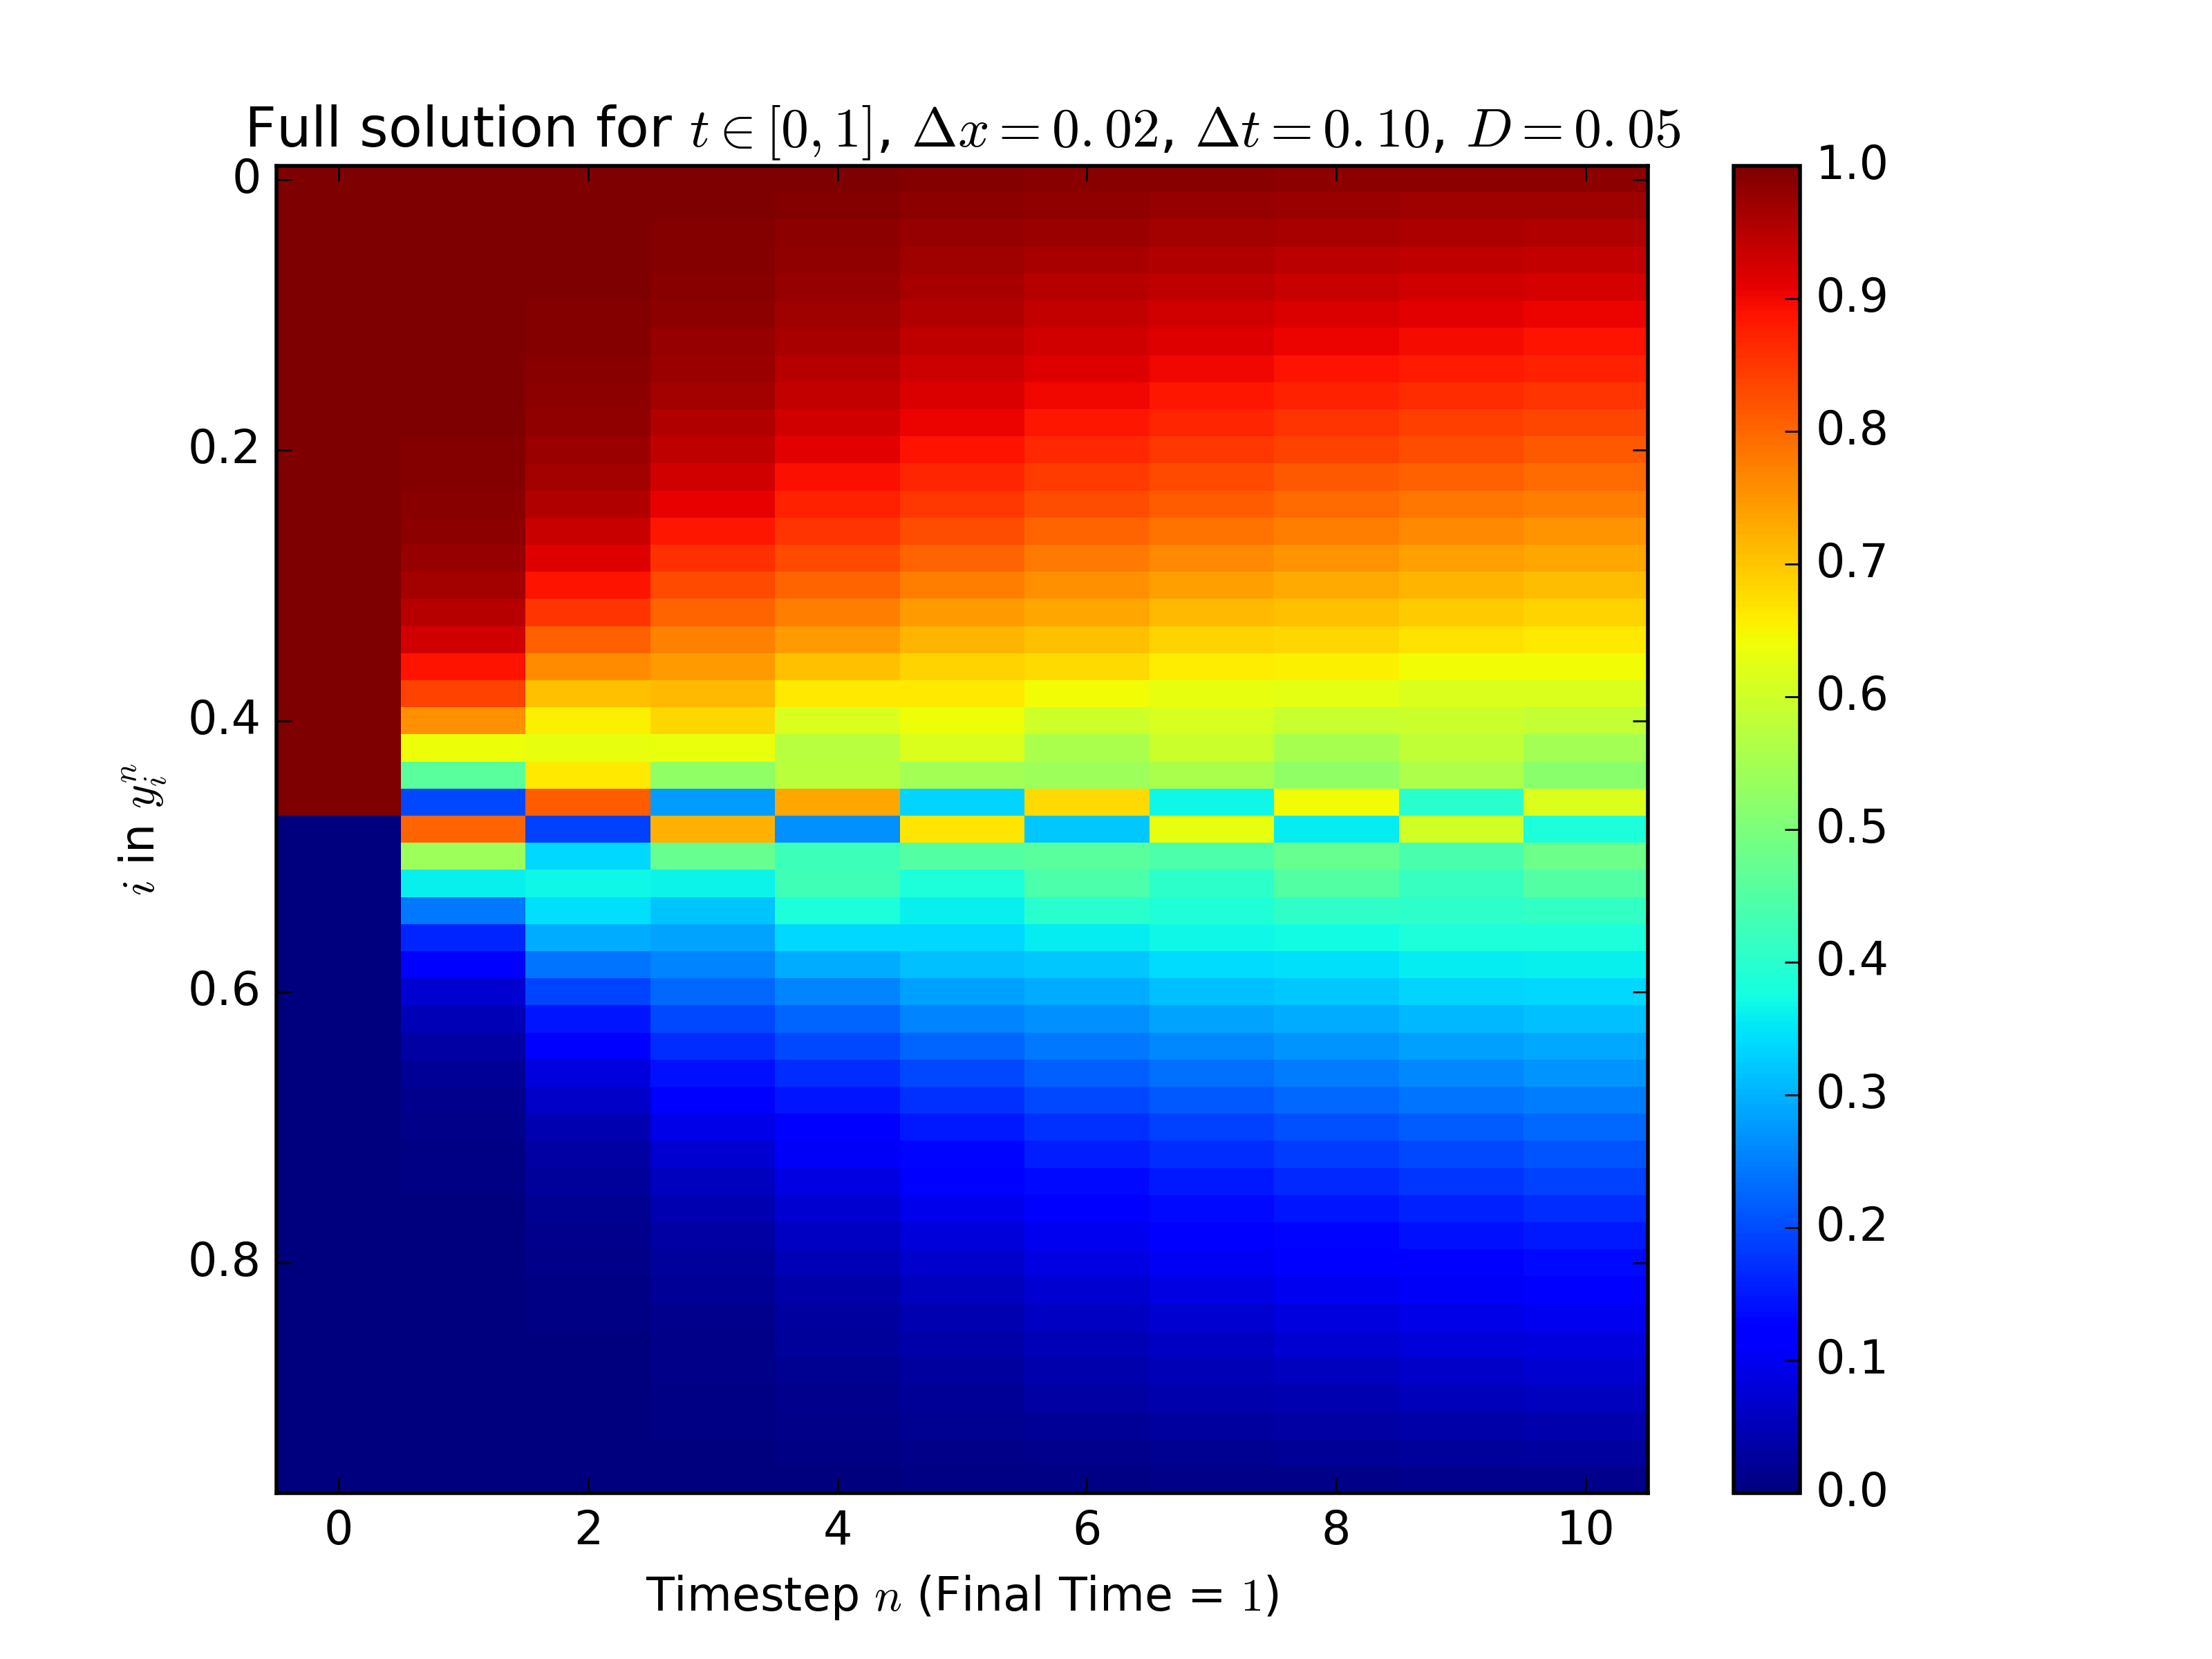
\includegraphics[width=\textwidth]{problem_3a_b.png}
    \end{minipage}
    This image on the left shows a $100\times$ decrease in timestep $\Dt$, and the strange oscillations practically disappear by $t = 1$.  The image on the right shows a $20\times$ decrease in the diffusion coefficient $D$, and the strange oscillations are almost completely gone by $t=1$.  These are clearly better than the large figure above, but certainly not sufficient to observe dynamics for $t \approx 0$.

    \item The Crank-Nicolson method for $u_t = Du_{xx} + f$ is
    \begin{align*}
        \frac{u_j^{n+1} - u_j^n}{\Dt} &= \frac{D}{2\Dx^2}\qty(u_{j+1}^{n+1} - 2u_j^{n+1} + u_{j-1}^{n+1} + u_{j+1}^n - 2u_j^n + u_{j-1}^n) + f \\
        -ru_{j+1}^{n+1} + \qty(1 + 2r)u_j^{n+1} - ru_{j-1}^{n+1} &= ru_{j+1}^n + (1 - 2r)u_j^n + ru_{j-1}^n
    \end{align*}
    where $r = \dfrac{D\Dt}{2\Dx^2}$.  So,
    \begin{align*}
        (I - rL)u^{n+1} &= (I + rL)u^n + \Dt f \\
        u^{n+1} &= (I - rL)^{-1}(I + rL)u^n + (I - rL)^{-1}\Dt f
    \end{align*}
    This is of the form $u^{n+1} = Bu^n + b$, where
    \begin{align*}
        B = \qty(I - rL)^{-1}\qty(I + rL)
    \end{align*}
    and
    \begin{align*}
        L = \qty[\begin{array}{ccccc}
            -2 & 1 & 0 & \dots & 0 \\
            1 & -2 & 1 & \dots & 0 \\
            0 & 1 & \ddots & \ddots & \vdots \\
            \vdots & \vdots & \ddots & -2 & 1 \\
            0 & 0 & \dots & 1 & -2
        \end{array}].
    \end{align*}
    The eigenvalues of $L$ are $\mu_k = -4\sin(k\pi \Dx)$ for $k = 1,\dots,N$, so the eigenvalues of $B$ are
    \begin{align*}
        \lambda_k = \frac{1 - \frac{2D\Dt}{\Dx^2}\sin(k\pi\Dx)}{1 + \frac{2D\Dt}{\Dx^2}\sin(k\pi\Dx)} \qquad \text{for }k = 1,\dots,N
    \end{align*}
    We know $-\mu_k$ ranges from near $0$ ($0 + \E$ for some small $\E>0$) to near $4$ ($4(1 - \delta)$ for some small $\delta$).  Then since $D = 1$, $\Dt = 0.1$, and $\Dx = 0.02$, $\frac{2D\Dt}{\Dx^2}\mu_k$ ranges from near $0$ ($500(0 + \E)$ for some small $\E$) to near $500$. ($500(1 - \delta)$ for some small $\delta$).  Thus for small $k$, $\lambda_k \approx 1$, and for large $k$, $\lambda_k \approx -1$ (in particular $\lambda \approx \frac{-499}{501}$).  This shows that the highest-frequency eigenvector, which is most represented near the initial discontinuity, has eigenvalue close to $-1$, which results in slowly decaying oscillations in time.  Also, a decrease of $D$ and $\Dt$ can still result in negative eigenvalues, but they have smaller magnitude than $\frac{-499}{501}$, which results in faster decaying oscillations in time.

    \item The BDF2 method for $u_t = Du_{xx} + f$ is
    \begin{align*}
        \frac{3u_j^{n+1} - 4u_j^n + u_j^{n-1}}{2\Dt} &= \frac{D}{\Dx^2}\qty(u_{j-1}^{n+1} - 2u_j^{n+1} + u_{j+1}^{n+1}) + f \\
        \qty(3I - rL)u^{n+1} &= 4u^n - u^{n-1} + 2\Dt f\\
        u^{n+1} &= 4\qty(3I - rL)^{-1}u^n - \qty(3I - rL)^{-1}u^{n-1} + 2\Dt\qty(3I - rL)^{-1}f
    \end{align*}
    where $L$ is given above and $r = \dfrac{2D\Dt}{\Dx^2}$.  This has the form $u^{n+1} = B_1u^n + B_2u^{n-1} + b$, where
    \begin{align*}
        B_1 = 4\qty(3I - rL)^{-1} \qquad\qquad \text{and} \qquad\qquad B_2 = -\frac{1}{4}B_1
    \end{align*}
    The eigenvalues of $B_1$ are
    \begin{align*}
        \lambda_k = \frac{4}{3 - r\mu_k}
    \end{align*}
    where $\mu_k$ are the eigenvalues of $L$ (given above).  Similarly, the eigenvalues of $B_2$ are $\sigma_k = -\frac{1}{4}\lambda_k$.  So, since $-\mu_k$ range from near $0$ to near $4$, and since $r = \dfrac{2(1)(0.1)}{(0.02)^2} = 500$, then the denominator of $\lambda_k$ range from near $3$ ($3 + \E$ for some small $\E$) to near $2003$ ($3 + 4(500 - \delta)$ for some small $\delta$).  This shows $\lambda_k$ range from near $\frac{4}{3}$ ($\frac{4}{3 + \E}$ for some small $\E$) to near $\frac{4}{2003}$ ($\frac{4}{3 + 4(500) + \delta}$ for some small $\delta$).  This shows that the eigenvalues of $B_2$ range from near $-\frac{1}{3}$ ($-\frac{1}{3 + \E}$ for some small $\E$) to near $-\frac{1}{2003}$ ($-\frac{1}{3 + 4(500) + \delta}$ for some small $\delta$).  So $\mu_k + \lambda_k$ range from near $1$ ($\frac{3}{3 + \E}$ for some small $\E$) to near $0$ ($\frac{3}{3 + 4(500) + \delta}$).  Since all these are positive and less than $1$, the dynamics should decay and not oscillate from timestep to timestep.

    Here is the backward Euler formulation, which is what should be used as the first step of BDF2:
    \begin{align}
        \frac{u_j^{n+1} - u_j^n}{\Dt} &= \frac{D}{\Dx^2}\qty(u_{j-1}^{n+1} - 2u_j^{n+1} + u_{j+1}^{n+1}) \\
        -ru_{j-1}^{n+1} + (1 + 2r)u_j^{n+1} - ru_{j-1}^{n+1} &= u_j^n
    \end{align}
    where $r = \dfrac{D\Dt}{\Dx^2}$.  This has the form
    \begin{align}
        u^{n+1} = Bu_j^n
    \end{align}
    where $B = (I - 2rL)^{-1}$ where $L$ is given above.
    Here are the results of my BDF2 code for $D = 1$, $\Dt = 0.1$, $\Dx = 0.02$:

    \begin{minipage}{\textwidth}
        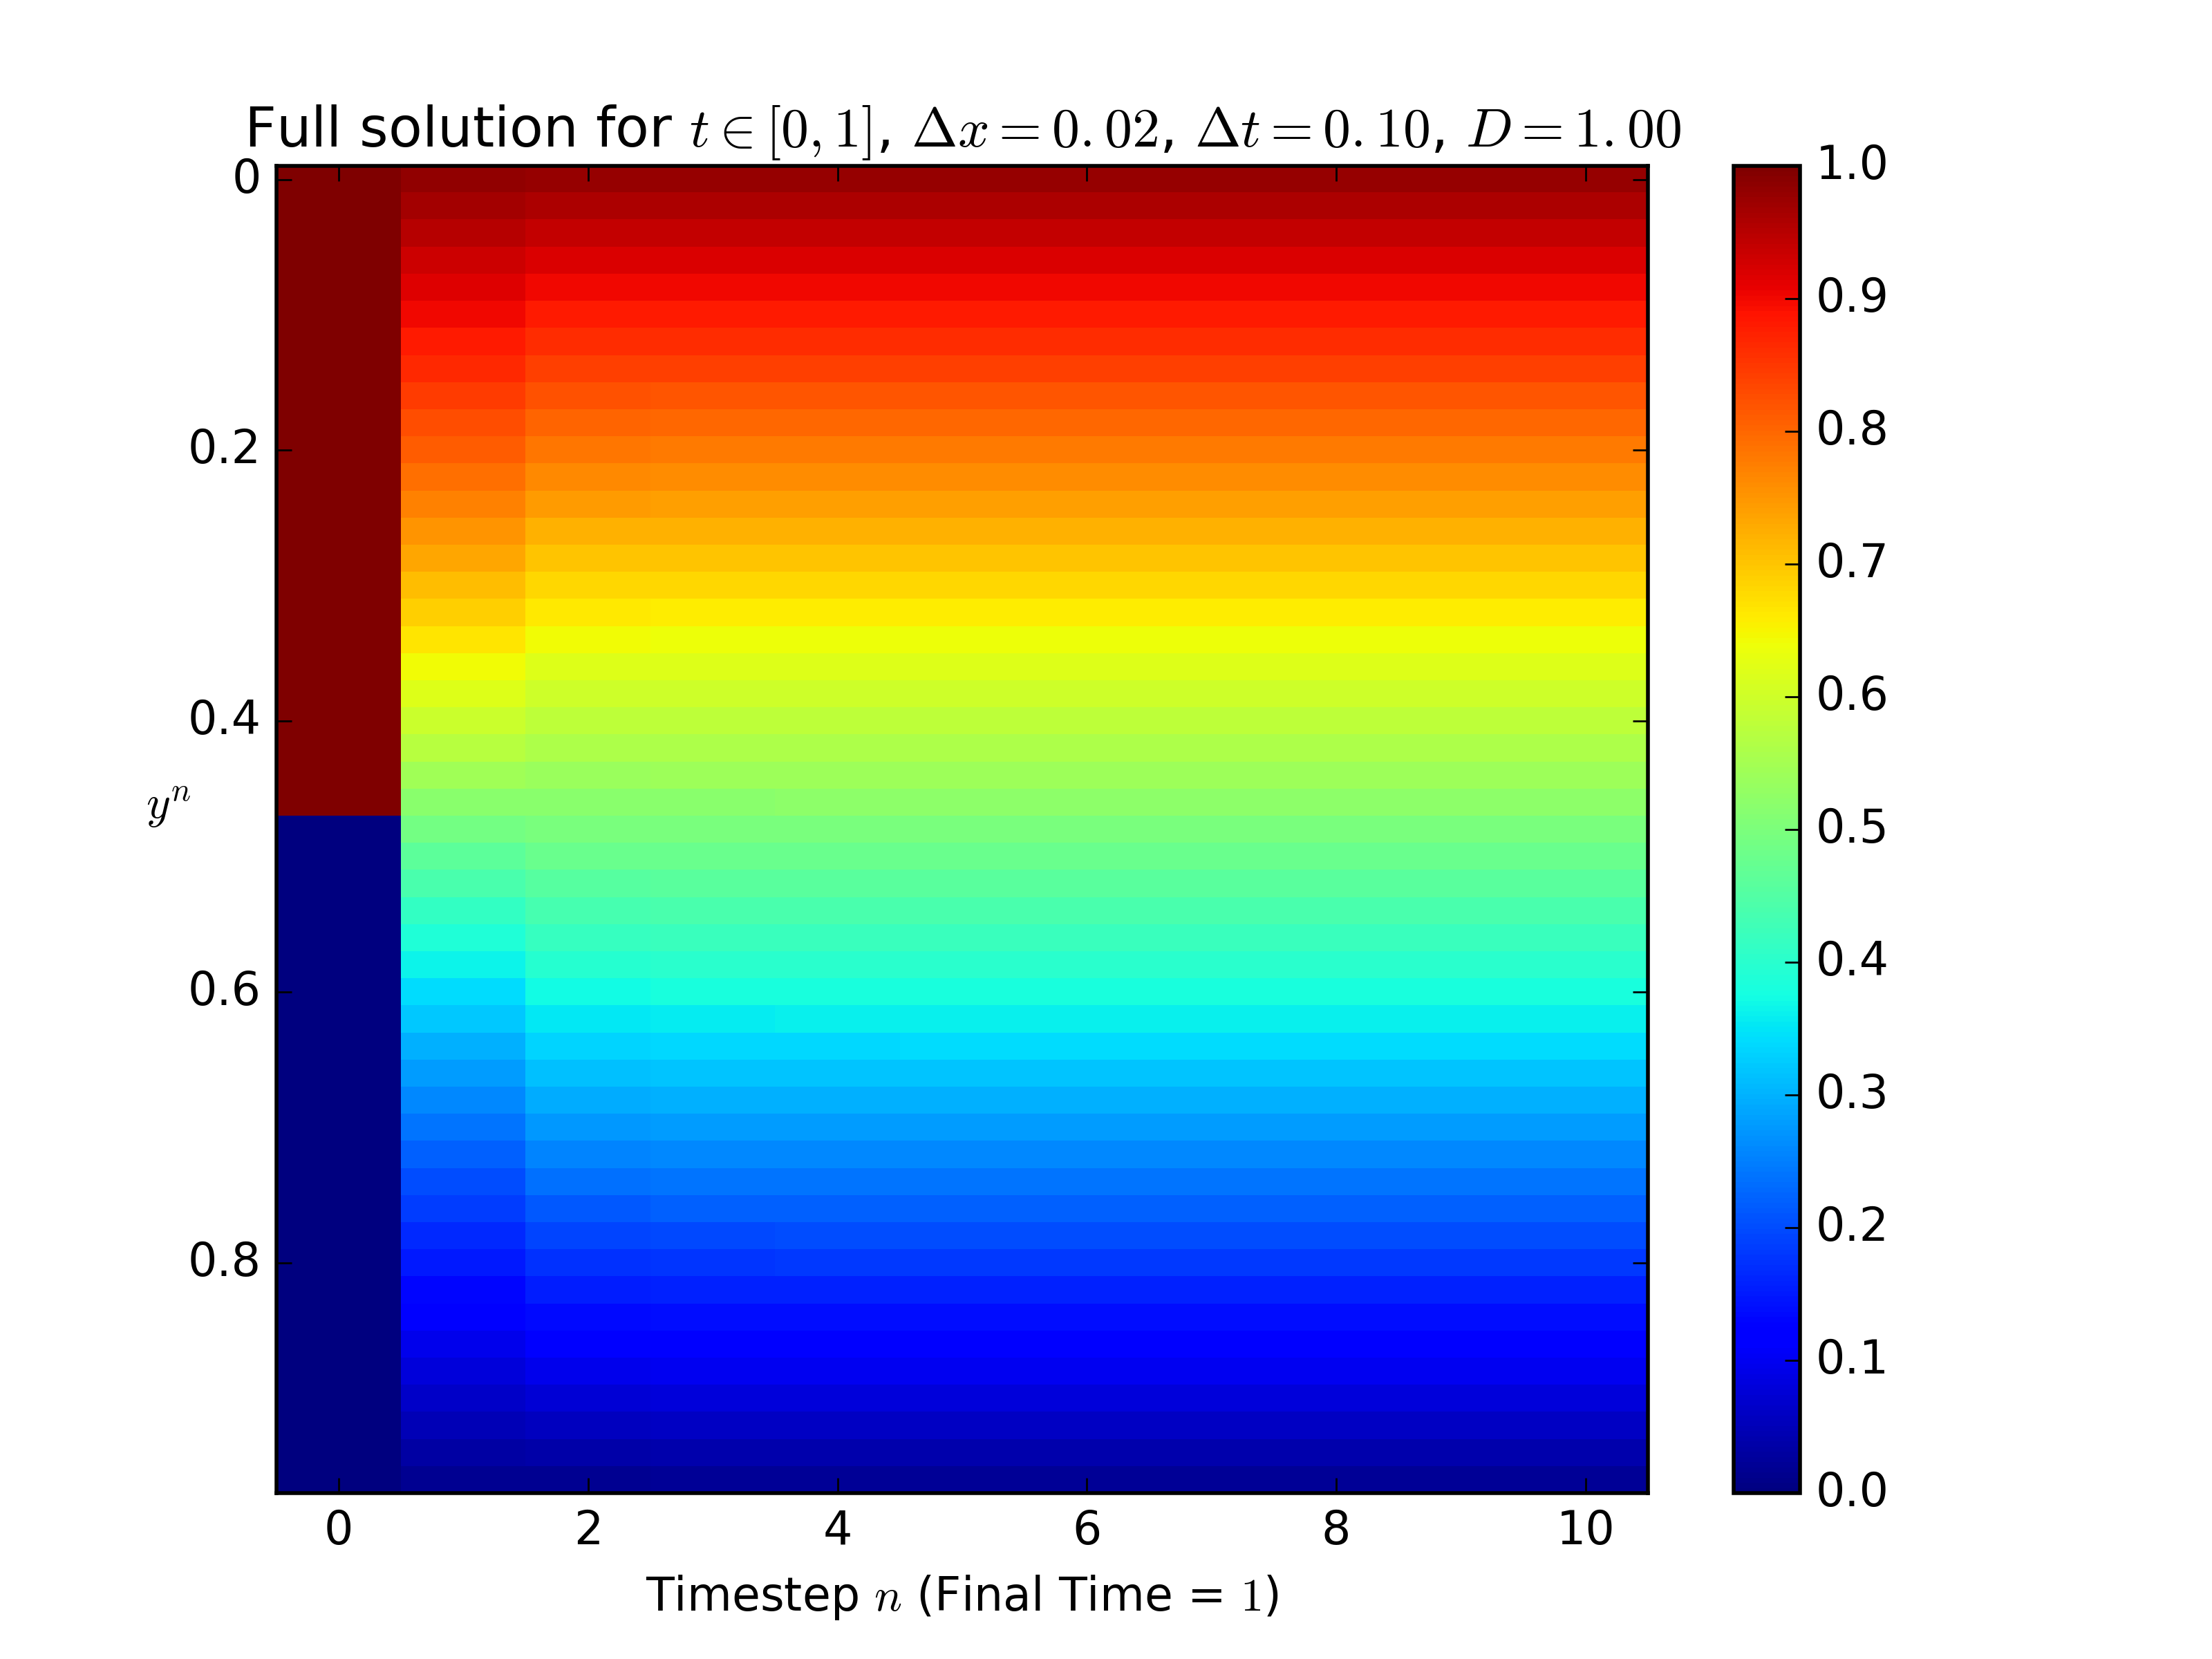
\includegraphics[width=\textwidth]{problem_3b.png}
    \end{minipage}
    Clearly this is a better solver than Crank-Nicolson for this type of problem.  Within only a few timesteps, equilibrium is reached.
\end{enumerate}

\end{document}









